\documentclass[12pt, a4paper]{memoir} % for a short document
\usepackage[french,english]{babel}

\usepackage [vscale=0.76,includehead]{geometry}                % See geometry.pdf to learn the layout options. There are lots.
%\geometry{a4paper}                   % ... or a4paper or a5paper or ...
%\geometry{landscape}                % Activate for for rotated page geometry
%\OnehalfSpacing
% \setSingleSpace{1.05}
%\usepackage[parfill]{parskip}    % Activate to begin paragraphs with an empty line rather than an indent


%===================================== packages
\usepackage{lipsum}
\usepackage{graphicx}
\usepackage{subcaption}
\usepackage{fullpage}
\usepackage{mathptmx} % font = times
\usepackage{helvet} % font sf = helvetica
\usepackage[utf8]{inputenc}
\usepackage{relsize}
\usepackage[T1]{fontenc}
\usepackage{tikz}
\usepackage{booktabs}
\usepackage{textcomp}%textquotesingle
\usepackage{multirow}
\usepackage{pgfplots}
\usepackage{url}
\usepackage{footnote}
\usepackage{amsmath,amssymb}
\usepackage{hyperref}
%============================================
\usetikzlibrary{arrows,shapes,positioning,shadows,trees}
\makesavenoteenv{tabular}
\makesavenoteenv{table}
%==============================================
\def\checkmark{\tikz\fill[scale=0.4](0,.35) -- (.25,0) -- (1,.7) -- (.25,.15) -- cycle;}
%Style des têtes de section, headings, chapitre
\headstyles{komalike}
\nouppercaseheads
\chapterstyle{dash}
\makeevenhead{headings}{\sffamily\thepage}{}{\sffamily\leftmark}
\makeoddhead{headings}{\sffamily\rightmark}{}{\sffamily\thepage}
\makeoddfoot{plain}{}{}{} % Pages chapitre.
\makeheadrule{headings}{\textwidth}{\normalrulethickness}
%\renewcommand{\leftmark}{\thechapter ---}
\renewcommand{\chaptername}{\relax}
\renewcommand{\chaptitlefont}{ \sffamily\bfseries \LARGE}
\renewcommand{\chapnumfont}{ \sffamily\bfseries \LARGE}
\setsecnumdepth{subsection}


% Title page formatting -- do not change!
\pretitle{\HUGE\sffamily \bfseries\begin{center}}
\posttitle{\end{center}}
\preauthor{\LARGE  \sffamily \bfseries\begin{center}}
\postauthor{\par\end{center}}
\newcommand{\jury}[1]{%
\gdef\juryB{#1}}
\newcommand{\juryB}{}
\newcommand{\session}[1]{%
\gdef\sessionB{#1}}
\newcommand{\sessionB}{}
\newcommand{\option}[1]{%
\gdef\optionB{#1}}
\newcommand{\optionB} {}

\renewcommand{\maketitlehookd}{%
\vfill{}  \large\par\noindent
\begin{center}\juryB \bigskip\sessionB\end{center}
\vspace{-1.5cm}}
\renewcommand{\maketitlehooka}{%
\vspace{-1.5cm}\noindent
\includegraphics[height=12ex]{./img/logo-uga.png}\hfill\raisebox{2ex}{
\includegraphics[height=14ex]{./img/logoINP.png}}\\
\bigskip
\begin{center} \large
Master of Science in Informatics at Grenoble \\
Master Informatique \\
Specialization \optionB  \end{center}\vfill}
% =======================End of title page formatting

\option{Data Science}
\title{Deep learning with Siamese networks for instance search or identification} %\\\vspace{-1ex}\rule{10ex}{0.5pt} \\sub-title}
\author{Matthias Kohl}
\date{June 20 (TODO), 2017} % Delete this line to display the current date
\jury{
Research project performed at LIG - MRIM \\\medskip
Under the supervision of:\\
Georges Quénot, Jean-Pierre Chevallet\\\medskip
Defended before a jury composed of:\\
Head of the jury (TODO)\\
Jury member 1\\
Jury member 2\\
}
\session{June \hfill 2017}
\setcounter{tocdepth}{4}
\setcounter{secnumdepth}{4}

%%% BEGIN DOCUMENT
\begin{document}
\selectlanguage{English} % french si rapport en français
\frontmatter
\begin{titlingpage}
\maketitle
\end{titlingpage}

%\small
\setlength{\parskip}{-1pt plus 1pt}

\renewcommand{\abstracttextfont}{\normalfont}
\abstractintoc
\begin{abstract}
Your abstract goes here... TODO
\end{abstract}
\abstractintoc

\renewcommand\abstractname{Acknowledgement}
\begin{abstract}
This work has been carried out in the context of the Guimuteic project funded by Fonds Européen de Développement Régional (FEDER) of région Auvergne Rhône-Alpes


I would like to express my sincere gratitude to .. for his invaluable assistance and comments in reviewing this report...
Good luck :)
TODO
\end{abstract}


\renewcommand\abstractname{R\'esum\'e}
\begin{abstract} \selectlanguage{French}
Your abstract in French goes here... TODO
\end{abstract}
\selectlanguage{English}

\cleardoublepage

\tableofcontents* % the asterisk means that the table of contents itself isn't put into the ToC
\normalsize

\mainmatter
\SingleSpace
%==============================CHAPTERS==================
% !TeX root = ../full_report.tex

\chapter{Introduction}
\section{Motivation}
The research presented here is motivated by the GUIMUTEIC project,
a collaborative project between industry and LIG. The
aim is to develop a smart audio-guide for touristic or cultural sites.
% TODO cite project/LIG/etc

In practice, the final product should offer an augmented reality
interface to the user, with information about the object or objects
the user is looking at.

One part of the development consists in finding ways of identifying
objects the user is looking at. There are multiple possibilities,
for example based on the geo-localization of the user and other sensors.
In our research, we focus on the recognition of objects based
only on visual clues.

\section{Research problem}
More specifically, we are interested in the following problem:
We are given a collection with reference images for each object,
or instance, to be recognized. The task is to develop a system that,
given an image of one of the instances, can decide which instance
the image represents. We assume that, on average, less than ten images
are available for each instance.
We will refer to this problem as instance retrieval in the following.

There are a few problems similar to instance retrieval. For one, there is
the image classification problem: we are given a collection of images
where each image is assigned a class, like dog or fridge.
The task is to develop a system that, given an image, decides which
class the image represents.
This problem is of course similar if we simply consider each instance
to be a separate class. However, in classification, we usually
assume to have many images per class: hundreds or even thousands.
This means our problem is closer to few-shots classification, where
only few images are available for each class.

Another similar problem is image retrieval. In image retrieval,
we are given a collection of reference images and a query image.
We aim to rank the reference images by similarity to the query image.
Usually, in image retrieval, reference images are not labeled or loosely
labeled and many images are irrelevant to the query image. The challenge
is to rank the most similar images on top.
Instance retrieval is related to image retrieval in that we aim to
develop a notion of similarity between images. However, in instance
retrieval, we do not care about the rank of the returned images, since
we only consider the highest ranked image, which should represent the
instance to retrieve.

% TODO possibly elaborate here

\section{Challenges}
For all of the problems described above, deep learning approaches
based on convolutional neural networks (CNNs) have recently obtained
the state-of-the-art results. One of the drawbacks of CNNs is that
they require large amounts of data to be trained.

In our research problem in particular, we do not
have large enough amounts of data available to fully train a CNN.
However, we aim to develop a system that can learn a descriptor
specific to the reference images,
as the system only needs to recognize and differentiate between
instances of that particular dataset. So the system should be tuned to
the dataset. Since we usually have less than ten images per instance,
this is an important challenge to overcome.

Another challenge comes from the nature of the datasets: we were not
able to find similar datasets in the literature, with only a few,
clean images, for each instance and many instances.
Common datasets in image retrieval like Oxford5k~\cite{philbin_object_2007},
Paris6k~\cite{philbin_lost_2008} or Holidays~\cite{jegou_hamming_2008}
contain many images per instance, but a lot of noise,
as they are used to evaluate whether a system can robustly retrieve the
correct images out of a set of random images.
This means that the approaches used for image retrieval datasets may
not work as well for instance retrieval.

\section{Contributions}
We made the following three major contributions:
\begin{enumerate}
    \item We analyze existing approaches to image retrieval, classification
    and determine their shortcomings in our problem setting.
    \item Based on these shortcomings, we propose a novel approach
    to improve results in our problem setting.
    \item We evaluate the novel approach and compare with other approaches.
\end{enumerate}

% !TeX root = ../full_report.tex

\chapter{State of the art}
\section{SIFT and bag-of-words}\label{sec:sift}
Until recently, the state of the art in image retrieval and matching
was based on the idea of
bag-of-words~\cite{philbin_object_2007,mikulik_learning_2013}.
The approach was introduced to image retrieval by Sivic and Zisserman
~\cite{sivic_video_2003} as well as Csurka et al.~\cite{csurka_visual_2004}.

The idea behind the approach is to represent an image as a histogram,
or collection of frequencies, of visual words. The visual words should
be small, representative patches of the images in the dataset.
Usually, these visual words are obtained in multiple steps. First,
local features are extracted and encoded. The most common feature used
is SIFT~\cite{lowe_distinctive_2004}, a 128-dimensional vector representing
scale-invariant features. Then, the features are extracted for all
images and clustered into clusters of similar features.
The representative for each cluster is the center of the cluster,
i.e. the mean of all features falling into that cluster.
Each image can then be represented as a histogram of the occurrences
of these representative features.
This histogram forms the image descriptor, which has as many dimensions
as there are representative features and clusters.

Finally, for image classification, a classifier can be learned from the
descriptors of all images in the dataset. On the other hand, for image
retrieval or matching, the descriptors can be directly matched against
each other, based on some similarity measure.
In both cases, it can be useful to use a different similarity measure
than the euclidean distance in the original descriptor space.
For classification, this is done by employing an SVM classifier with a
non-linear kernel~\cite{shawe-taylor_kernel_2004}.
Among the most popular kernels are the
radial basis function~\cite{scholkopf_comparing_1997}
and the chi-squared function~\cite{vedaldi_efficient_2012}.

Until recently, this approach has obtained state-of-the-art results for
image retrieval tasks~\cite{mikulik_learning_2013}.

\section{Fisher vectors (FV)}\label{sec:fv}
The Fisher vector representation is based on the Fisher kernel, as described
by Jaakkola and Haussler~\cite{jaakkola_exploiting_1999}. The main idea
in their work is to derive a kernel function for discriminative classification,
where the kernel function is derived from a generative probability model.
For this, the log-likelihood with respect to a parameter $\log P(X|\theta)$
is considered, where $X$ is the data and $\theta$ the parameter.

The Fisher vector is based on the gradient of this log-likelihood which
essentially captures how much the parameter contributes to the generation
of a sample $X$. This principle has been applied to images as well by
Sanchez et al.~\cite{sanchez_image_2013}, in the context of image
classification. Here, the data (or samples) are the local descriptors of
patches of images and the parameters to be estimated are the parameters
of a Gaussian Mixture Model (GMM) of these descriptors.
This means that we consider the descriptor of an image as a
combination of local descriptors, each being independent of all others,
with each local descriptor contributing to the global descriptor through
a GMM. This GMM can have any number
of parameters, which can be learned through the expectation maximization
algorithm. The Fisher vector is the gradient of the log-likelihood of this
GMM with respect to the parameters. Thus, it represents the combination
of deviations from the generative model of all local descriptors of the
image, for each parameter of the model.

Another important property is that the Fisher
vector embeds each local descriptor into a space of
different dimension, which consists of the parameters of the GMM:
weights, means and co-variances of the Gaussians.
The dimensionality of the Fisher vector is thus ultimately dependent
on the number of Gaussians chosen for the GMM.

It can be shown that this representation represents a kernel for a kernel
machine and can thus be used very efficiently by linear classifiers learning
their parameters in the Fisher kernel space.

While the Fisher vector representation has a high dimensionality, it
has been shown that it can be compressed efficiently
~\cite{sanchez_image_2013,perronnin_large-scale_2010} and can be applied
to large-scale image retrieval systems~\cite{perronnin_large-scale_2010}.

\section{VLAD}
Another important descriptor used in image retrieval systems is the
vector of locally aggregated descriptors or VLAD. It was introduced
by Jegou et al.~\cite{jegou_aggregating_2010} and is related to both
the bag-of-words and the Fisher vector representations described in
Sections~\ref{sec:sift}~and~\ref{sec:fv}.

As with the bag-of-words approach, a visual vocabulary is formed
using the k-means clustering algorithm. Then, for each visual
word $w$ (one of the $k$ centers of the output of k-means)
and each local descriptor $x$ associated with $w$ (where $w$ is the closest
center), the difference $x-w$ is added to the VLAD representing $w$.

Hence, VLAD is a sum over the differences between all local descriptors
and their associated visual word. This is similar to the Fisher vector
representation, which represents a sum of the deviations of local
descriptors from the generative model, which can be seen as consisting
of the visual vocabulary.

Jegou et al.~\cite{jegou_aggregating_2010} show that the VLAD representation
has many advantages over previous representations. For one, it achieves
state-of-the-art results on the Holidays dataset~\cite{jegou_hamming_2008}.
Furthermore, it can be compressed efficiently using principal component
analysis and still achieve promising results, making it faster to
compute than the Fisher vector representation, even when compressed
as described in Section~\ref{sec:fv}.

\section{Deep learning with CNNs}
Starting with the results of AlexNet for image classification in the 2012
ImageNet challenge~\cite{krizhevsky_imagenet_2012,russakovsky_imagenet_2015},
image classification tasks have been dominated by CNNs, learned using
large amounts of data.

A general trend in image related tasks is to move to an end-to-end
approach, where the final objective is directly optimized using gradient
descent and the gradient is back-propagated to all previous parts of the
system. In contrast, the bag-of-words model requires a choice of
features (SIFT, ORB~\cite{rublee_orb:_2011}, \dots),
a choice of the method for clustering features (k-means),
a choice of the classifier (AdaBoost~\cite{freund_desicion-theoretic_1995},
SVM, \dots), as well as a choice of the kernel if an SVM classifier is used.

Using a CNN, features are extracted at a low abstraction level by the
first convolutional layers, then higher level features are formed
by combining low level features from the previous layers. Finally,
high-level features are combined into a classifier by linear layers.
All layers are then optimized together, usually through three main steps.
First, a loss function evaluates the loss made by the last layer of
the network. Then, the back-propagation algorithm
~\cite{rumelhart_learning_1988} exploits the chain-rule of derivatives
to propagate the gradients of the errors made by each layer from the
last layer to the first layer of the network. Finally, a stochastic
gradient descent algorithm
~\cite{bottou_stochastic_2012,bottou_large-scale_2010,rumelhart_learning_1985}
is used to optimize the parameters of all layers with respect to the loss.
The advantage of this approach is that the features are learned at all
abstraction levels at once. Another advantage of neural networks is their
modularity. It allows us to easily transfer the lower level features
learned from a large dataset to a smaller dataset, where there may not
be sufficient amounts of data to efficiently learn lower level features.

The following sections describe the high-level architecture of the
most widely used CNNs in classification and image retrieval.
\subsection{AlexNet}
AlexNet~\cite{krizhevsky_imagenet_2012} contains five convolutional
layers and three linear layers. The first convolutional layer
has a large kernel and stride to quickly increase the receptive field
of the consequent filters. The first two convolutional layers are followed
by a pooling layer to further increase the receptive field.

Finally, an important improvement for AlexNet to avoid over-fit is
the addition of dropout layers~\cite{hinton_improving_2012} before the
two first linear layers.

Apart from that, AlexNet is a simple adaptation of LeNet by
LeCun et al.~\cite{lecun_gradient-based_1998} for the ImageNet challenge.

\subsection{VGG}
The VGG architecture, introduced by
Simonyan and Zisserman~\cite{simonyan_very_2014}
is the first to use exclusively $3\times3$ convolutional kernels.
This means that the receptive field of the
first filters is much smaller, and thus many more layers are needed,
as well as more pooling layers. The most popular VGG architectures
are VGG-16 and VGG-19, having 16 and 19 layers in total respectively.

Using smaller kernels in convolutions and consequently more layers
allows to reduce the number of trainable parameters used by the
network, while increasing the number of non-linear layers.
This was shown to allow better generalization properties, and thus less
over-fit~\cite{simonyan_very_2014}.

\subsection{ResNet, Inception, DenseNet}\label{sec:verydeepCNNs}
The idea of increasing the number of layers is further developed
by the ResNet, DenseNet and Inception architectures. However,
naively increasing the number of layers leads to the problem of
vanishing gradient~\cite{hinton_fast_2006}.

All of these networks overcome the vanishing gradient problem by
introducing skip connections, where the output of a previous layer
is added to the output of a layer, skipping some number of layers in
between.

The ResNet architecture by He et al.~\cite{he_deep_2016} always uses blocks
of 3 layers along with a skip of those 3 layers. The smaller types of
ResNet use blocks of 2 layers.

The Inception architecture by Szegedy et al.~\cite{szegedy_inception-v4_2016}
uses a combination of skip connections of different length and different
types.

Finally, DenseNet by Huang et al.~\cite{huang_densely_2017} takes the
skip connection idea one step further:
the input of each layer is dependent on the output of all $n$ previous layers
to some extent.

All of the very deep architectures use batch norm layers after the
convolutional layers to further reduce over-fit~\cite{ioffe_batch_2015}:
a batch norm layer simply normalizes the features over each
batch, and then applies a learn-able scaling and shifting. During training,
it also produces estimates of the over-all mean and variance of the input
of the layer over the whole dataset.
These estimates of the global mean and variance are used during evaluation
in order to normalize the data after each block of convolutional and
pooling layers.

\section{Image retrieval using CNNs}
For image retrieval, the current state of the art is set by
Gordo et al.~\cite{gordo_deep_2016}. It is based on an
end-to-end approach. The goal is to learn a global descriptor for images
that is well suited for comparing images.

\begin{figure}
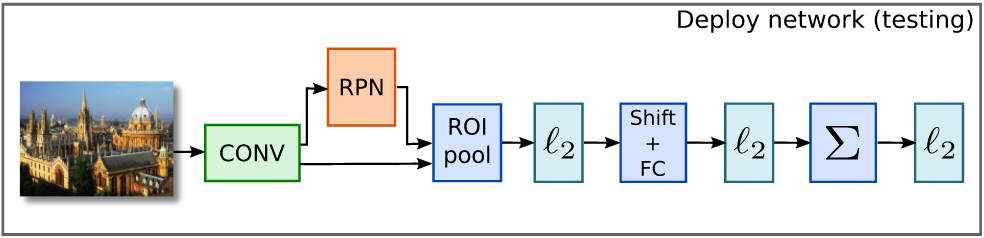
\includegraphics[width=\textwidth]{img/gordo_deepimageretrievaldeploy.png}
\caption{Architecture of a CNN network for image retrieval, developed by
Gordo et al.~\cite{gordo_deep_2016}
\label{fig:gordo_deploy}}
\end{figure}
Figure~\ref{fig:gordo_deploy} shows the detailed architecture used.
It first extracts the convolutional features of a pre-trained
CNN. Then, a Region Proposal Network (RPN)~\cite{ren_faster_2015} is
used to extract the regions of interest. For each region of interest,
a shifting layer, followed by a linear layer are used to reduce the
dimensionality of the descriptor.
The final descriptor consists of a normalized sum of the
region-wise descriptors. This network can be learned end-to-end and
the obtained descriptor achieves state-of-the-art results, which can
be even further improved by using query expansion and database side
feature augmentation (described in detail in Section~\ref{sec:improvedesc}).

Gordo et al.~\cite{gordo_deep_2016} found that using very deep networks
outperforms the shallower networks. The state-of-the-art results are
thus set by a very deep ResNet-50 architecture, using 50 layers.

\subsection{Siamese networks and triplet loss}
\begin{figure}
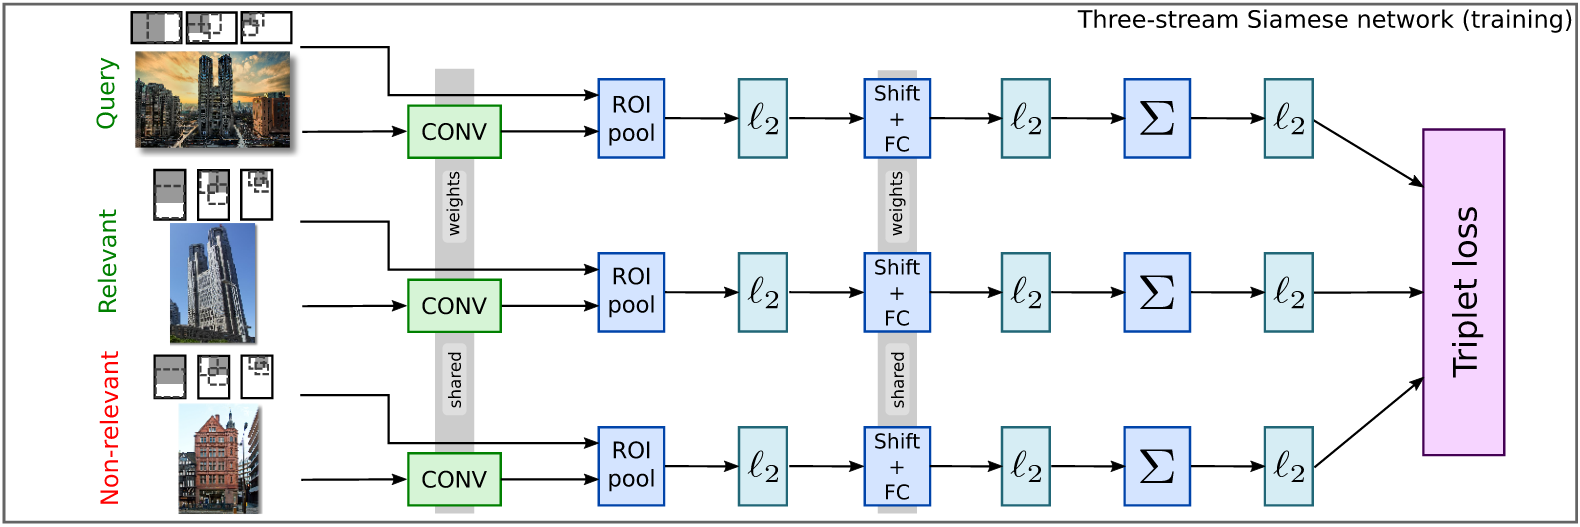
\includegraphics[width=\textwidth]{img/gordo_deepimageretrievalarc.png}
\caption{Siamese architecture of a CNN for image retrieval used in
training~\cite{gordo_deep_2016}
\label{fig:gordo_train}}
\end{figure}

Figure~\ref{fig:gordo_train} shows the architecture used to train the CNN
that produces a descriptor for images, as can be seen in
Figure~\ref{fig:gordo_deploy}.

The major difference is that during training, a Siamese architecture is
used: the CNN is evaluated with multiple images, using the same weights
for each. Then, a combined loss is obtained from the descriptors.
Finally, the loss is back-propagated once through all streams of the network,
since shared weights are used for all images.

The Siamese architecture was first proposed by Chopra et al.
~\cite{chopra_learning_2005} in the context of facial recognition.
In this paper, pairs of images are used and a loss was designed to
move the descriptors of a pair of images together in the descriptor space,
if the pair represents the same face, while separating the descriptors
if they represent different faces.

In the case of the architecture presented in Figure~\ref{fig:gordo_train},
three images are evaluated and a triplet loss is used.
This triplet loss was shown to be more robust during training than a
loss using pairs and has been used to set the state of the art
in facial recognition tasks by Schroff et al.~\cite{schroff_facenet:_2015}.
The triplet loss was first introduced by
Weinberger et al.~\cite{weinberger_distance_2006} as a way of learning
the best suited distance metric in a k-nearest neighbor classification
problem through gradient descent.
This is the reason why the triplet loss was chosen for image retrieval:
the goal is to learn a metric which allows to discriminate couples of
images containing the same instance from couples of images containing
different instances, using the descriptors obtained from the deep
CNN.
Section~\ref{sec:tripletloss} describes this loss in more detail.

Finally, Gordo et al. made further contributions, detailed in their
follow-up paper~\cite{gordo_end--end_2017}. These contributions are
presented in the following sections.

\subsection{Dataset}
For one, an important step is to use a suitable dataset. Datasets like
Oxford5k or Paris6k are too small for a network to learn a distance metric
applicable to any type of image. Instead, the state of the art uses the
much larger Landmarks dataset, created by Babenko et al.
~\cite{babenko_neural_2014} for training.
This dataset contains almost 200000 images in total, of around 600
different landmarks, mostly buildings.

Another important step is the cleaning of the dataset. The Landmarks
dataset contains a lot of noise and weak labels: many images do not
represent the building they are labeled with. Gordo et al.
~\cite{gordo_end--end_2017} use a meticulous
cleaning process: the main idea is to keep only the largest clusters
of matching objects for each of the landmarks. The implementation is
based on extracting SIFT and Hessian descriptors,
matching them and verifying matches with an affine transformation model.
This cleaning process is used in order to annotate the cleaned images
with regions of interest as well.

The cleaning requires a lot of processing,
but is only done once for the dataset.
The cleaned dataset is still fairly large, containing 49000 images and
586 instances of landmarks.

\subsection{Triplet selection}
Another important step is the selection of triplets during training of
the Siamese network. In a nutshell, choosing random triplets for training means that most triplets do not contribute to the loss at all,
thus leading to vanishing gradients
~\cite{schroff_facenet:_2015,weinberger_distance_2006}.

Thus, different methods have been proposed to overcome this problem
~\cite{gordo_end--end_2017,schroff_facenet:_2015}. These methods
aim at choosing the hardest triplets, contributing the most to the loss.
This needs to be done without being computationally too expensive
nor choosing exclusively the hardest triplets, as this can collapse
the model early on in training~\cite{schroff_facenet:_2015}.

The different triplet selection mechanisms are detailed and discussed
in Section~\ref{sec:tripletselection}.

\subsection{Limitations and goals}\label{sec:limitations}
The main limitation of the state of the art with respect to instance retrieval
is that it aims at producing a general descriptor for comparing any type
of image. This means that it
is most effective when trained on large datasets, with many samples
per instance. For datasets containing images from museums or tourist
sites, this is usually not applicable, as there are usually only very few
images available for each instance. While there are large datasets,
these datasets usually contain a large number of instances as well.
This makes it difficult to directly apply the state of the art on
our datasets.

On the other hand, it also means that the state of the art in
image retrieval aims at avoiding over-fit at all costs:
the learned descriptor and metric should
be able to provide a good metric for any kind of image.
While this is usually desired in machine learning, in our case,
one goal is to provide a metric specifically designed
to discriminate between the images of the given dataset. This is because
an audio-guide in a museum can be fine-tuned for that museum, as long
as the fine-tuning is computationally cheap enough. So we do not care
if a given audio-guide cannot identify images of multiple museums,
as long as it can identify images of one museum with high precision.

Another limitation of the state of the art is that it requires
a tedious process to clean the dataset and annotate it with regions of
interest. This is not suited to museum datasets which are usually very
clean to begin with, by the nature of the dataset. Plus, the notion of
region of interest is usually not relevant for this type of image:
which part of a painting or piece of art contains the semantically
relevant information is not obvious.

Finally, an evaluation of the state-of-the-art network~\cite{gordo_deep_2016}
was carried out.
We used the published weights obtained in training this CNN on the
Landmarks dataset.
Figure~\ref{fig:incorrectimg}
shows examples of images in our dataset that were correctly matched
with high confidence as well as images that were incorrectly matched.
From these images, we make the following observations in
Section~\ref{sec:incorrectimages}:

\begin{enumerate}
    \item Images that are very similar visually are well matched
    \item Images at different scales are not well matched
\end{enumerate}

Thus, a limitation of the current state of the art is matching
images, where the object of interest is at different scales.

The goal for our research is thus to try to overcome the limitations
of the current state of the art by proposing a descriptor which can
be fine-tuned to each dataset, is robust to differences in scale and
does not require annotations of regions of interest.

% !TeX root = ../full_report.tex

% TODO possibly images showing saliency map/feature map of filter
% before and after fine-tuning

\chapter{Contributions}
\section{Fine-tuning a CNN}\label{sec:finetuning}
A first possible approach to this problem is to fine-tune
a classification network to instance classification. This means that
we consider each instance as a class, and optimize using a cross-entropy
loss, typical for classification.

\begin{equation}\label{eq:crossent}
\mathcal{L} = - \frac{1}{N}
\sum_{i=1}^N y_i \log \hat{y}_i + (1-y_i) \log (1-\hat{y}_i)
\end{equation}

Equation~\ref{eq:crossent} describes the cross-entropy loss for a
given instance. $N$ is the number of samples, $y_i$ an indicator
variable taking the value $1$ if sample $i$ belongs to the given
instance and $0$ otherwise, and $\hat{y}_i$ is the predicted probability
that sample $i$ belongs to the given instance.

Fine-tuning a CNN for classification on different data has been studied
intensively by Yosinki et al.~\cite{yosinski_how_2014}. In particular,
their study shows that it is only important to fine-tune the neurons
of higher layers of a CNN. Furthermore, they show that
fine-tuning can increase generalization even in the fine-tuned model.
Both of these properties are desirable in our task, because they reduce
the memory and time needed to train a network, as well as the need
for a large dataset used for fine-tuning.

The specific considerations we take with regards to fine-tuning are
described in the following sections.

\subsection{Data augmentation}
Our datasets, presented in Section~\ref{sec:datasets},
contain an average of less than 10 samples per instance. This is too little
to train a typical CNN model designed for classification, even when
fine-tuning.
One way to overcome this is to augment the data, by randomly applying
affine transformations, color perturbations and other random transformations.
% TODO possibly reference some paper here

Since we specifically identified an issue related to different scales
in images in Sections~\ref{sec:limitations}~and~\ref{sec:incorrectimages},
it it natural to augment the data by randomly scaling the images in both
dimensions.

We found that randomly rotating and flipping the images improved
performance as well, thus we perform this type of data augmentation
throughout our experiments.

For data augmentation in order to fine-tune a CNN, we use the
following values in our experiments:
\begin{enumerate}
    \item Rotation: any angle is chosen with the same probability.
    \item Scaling: the scaling factor is chosen independently for each
    dimension in the range $[0.75,1.25]$.
    \item Flipping: with probability $0.5$, images are horizontally
    flipped.
\end{enumerate}

\subsection{Transfer learning}
The modularity of a CNN means that we can easily transfer
the weights from a pre-trained model, and only retrain the highest
abstraction layers. Specifically, we re-train all linear layers in the
model, representing the highest-level layers.

We also re-train the highest level convolutional layers, since our datasets
contain many visually different images as compared to the ImageNet
dataset used for pre-training the models.
For the AlexNet architecture, we choose to re-train all layers above
and including the last convolutional layer.
For a ResNet architecture, we re-train all layers above and including the
third to last block of convolutional layers. This contains the
nine highest convolutional layers in total.

\section{Simplified Siamese architecture}\label{sec:simplifiedsiam}
We follow the methodology of Gordo et al.~\cite{gordo_deep_2016} and
propose a simplified Siamese architecture. As shown in
Figure~\ref{fig:gordo_train}, the previous state-of-the-art is set
by a Siamese architecture using the triplet loss.

\subsection{Triplet loss}\label{sec:tripletloss}
\begin{equation}\label{eq:tripletloss}
\mathcal{L} = \sum_{i=1}^N \frac{1}{2}
\max(0, \|x^a_i - x^p_i\|_2^2 - \|x^a_i - x^n_i\|_2^2 + 2m)
\end{equation}

Equation~\ref{eq:tripletloss} describes the triplet loss for $N$
triplets. Each triplet is composed of an anchor image with descriptor
$x^a$, a positive/relevant image with descriptor $x^p$ and a
negative/non-relevant image with descriptor $x^n$. A margin $m$ is added
to the loss, which describes the distance at which two images are
considered similar enough to be relevant with respect to each other.
Throughout our experiments, this margin is set to a value of $m=0.1$.

For normalized descriptors $x$ and $y$, the squared distance $\| x - y \|_2^2$
is closely related to the cosine similarity and the dot-product through
the relationship derived in Equation~\ref{eq:sqdistcosdot}.

\begin{equation}\label{eq:sqdistcosdot}
\begin{array}{ll}
\multicolumn{2}{l}{\forall x, y \in \mathbb{R}^n, \|x\|_2 = 1, \|y\|_2 = 1}\\
\|x-y\|_2^2 &= (x_1-y_1)^2 + \dots + (x_n-y_n)^2\\
&=(x_1^2 + \dots + x_n^2) - 2(x_1y_1 + \dots + x_ny_n) +
(y_1^2 + \dots + y_n^2)\\
&=2 - 2xy = 2 - 2\cos(x, y)
\end{array}
\end{equation}

With this Equation, we can re-write the triplet loss for normalized descriptors
using the dot-product, as shown in Equation~\ref{eq:tripletlossnorm}.
This equation represents the version of the triplet loss used in
our experiments. This means all descriptors must be normalized before
the loss is evaluated.

\begin{equation}\label{eq:tripletlossnorm}
\mathcal{L} = \sum_{i=1}^N
\max(0, x^a_i x^n_i - x^a_i x^p_i + m)
\end{equation}

\subsection{Simplified architecture}
We simplify the architecture shown in Figure~\ref{fig:gordo_train}
by removing the region proposal network and region of interest pooling.
We justify in Section~\ref{sec:roi} why these components are not
relevant for our datasets and research problem in general.
Except for this change, the architecture is kept exactly as described
by Figures~\ref{fig:gordo_deploy}~and~\ref{fig:gordo_train}.

\subsection{Triplet selection}
As noted by previous authors, when using the triplet loss, it is
crucial to choose the best triplets during training in order to
obtain convergence. In particular, many triplets are irrelevant
and do not produce any loss since they are \emph{too easy} for the network.

Hence, the first idea is to choose the hardest triplets, as proposed by
Schroff et al.~\cite{schroff_facenet:_2015}. However, as they show in
their paper, this can lead to a collapsing model early on in training
so they choose  \emph{semi-hard} triplets instead. Semi-hard triplets
are obtained as follows:
use all possible positive couples of images: couples of images from the
same instance. For each positive couple, choose the hardest negative
that is easier than the positive couple. Hard and easy are defined
by the dot-product between the descriptors of the images: a high value
of the dot-product for images of the same instance represents an easy
positive couple, a high value of the dot-product for images of different
instances represents a hard negative couple.
The value of all dot-products are determined before each pass over
the whole training data during training, for all couples of images.

Gordo et al.~\cite{gordo_end--end_2016} propose a more complex mechanism.
First, they also calculate the values of dot-products for all couples of
images before each pass over the training data.
Second, for each image, choose the $n$ easiest positive images and the
$m$ hardest negatives. Then, calculate the loss for all possible combinations
and use the $o$ triplets with the highest loss.
This method probably eliminates some noise when choosing the easiest
positive couples, for images that are labeled as being the same instance
but are not visually similar.
However, in experiments, we found that this method does not perform well
for datasets with few images per instance, since we either have to
choose $n$ as very low or we choose all positive couples after all for
most instances.

Hence, in our experiments, we choose the semi-hard triplet selection
for the first two passes over the dataset, after which we only choose
the hardest negatives for all positive couples.

\section{Region of interests and object localization}\label{sec:analysisprev}
\subsection{Identifying regions of interest}\label{sec:roi}
Previous approaches in image retrieval
~\cite{gordo_end--end_2016,salvador_faster_2016,tolias_particular_2015}
usually deal with regions of interest in one way or another.
The idea is that in most cases, only certain parts of each image can
be useful for comparison with other images. In addition to this,
cropping images at their regions of interest can help with differences
in scale of the images to compare: if a building is visible only in a small
part of an image, cropping the image at that part and then re-scaling
the part should set the building at a normalized scale.

However, in instance search with museum datasets, it is not obvious
where the regions of interest should be: most images represent an entire
painting or parts of it and only some may contain the painting as part
of the image with a wall in the background. This means for most images,
the ground-truth region of interest is simply the entire image, and some
may have a ground-truth region of interest which is almost the entire image,
excluding only a small part of the background.

On the other hand, a network fine-tuned on classification on such a dataset
should be able to easily identify the region containing the painting, since
the background wall is contained in almost all classes, which means it is a
particularly bad indicator of the class. Thus, if the network is applied in
a strided manner across an image, it should produce low maximal activations
in parts containing big sections of background wall.

\begin{figure}
\centering
\begin{subfigure}[b]{0.3\textwidth}
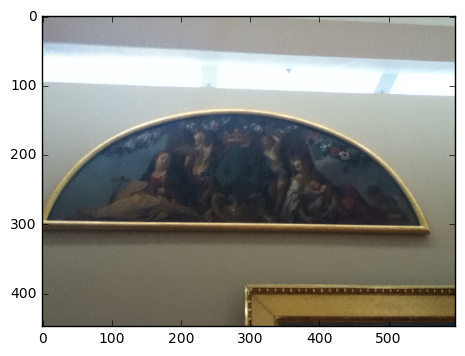
\includegraphics[width=\textwidth]{img/sample1_10A-0519.png}
\caption{Image with label 10A\label{fig:sample1_id}}
\end{subfigure}
\begin{subfigure}[b]{0.3\textwidth}
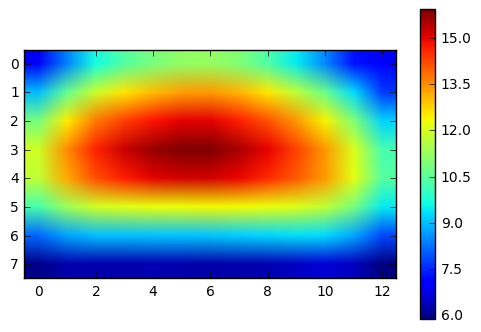
\includegraphics[width=\textwidth]{img/sample1_heatmap.png}
\caption{Heat-map for 10A\label{fig:sample1_hm}}
\end{subfigure}
\begin{subfigure}[b]{0.3\textwidth}
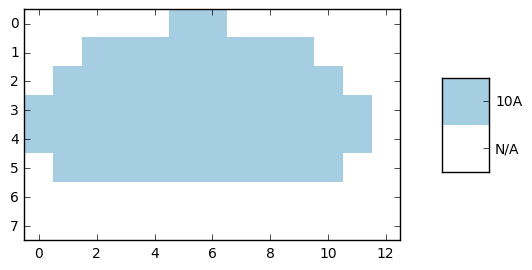
\includegraphics[width=\textwidth]{img/sample1_labels.png}
\caption{Label-map for 10A\label{fig:sample1_lab}}
\end{subfigure}

\begin{subfigure}[b]{0.3\textwidth}
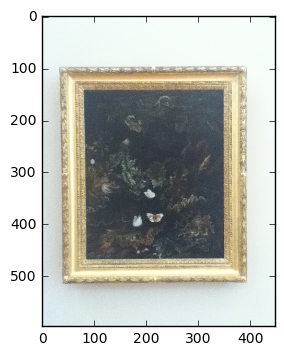
\includegraphics[width=\textwidth]{img/sample2_5P-0508.png}
\caption{Image with label 5P\label{fig:sample2_id}}
\end{subfigure}
\begin{subfigure}[b]{0.3\textwidth}
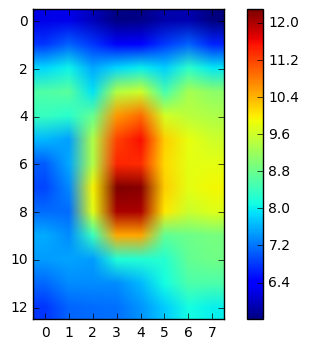
\includegraphics[width=\textwidth]{img/sample2_heatmap.png}
\caption{Heat-map for 5P\label{fig:sample2_hm}}
\end{subfigure}
\begin{subfigure}[b]{0.3\textwidth}
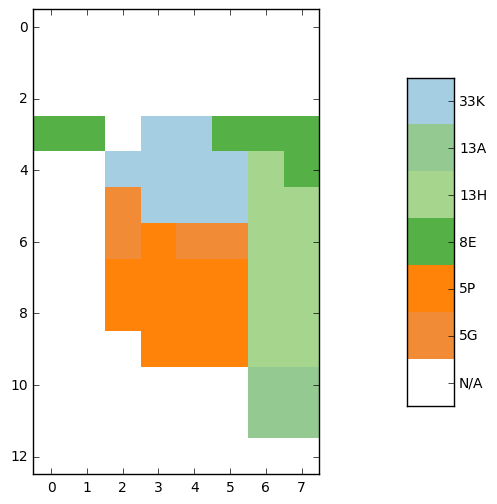
\includegraphics[width=\textwidth]{img/sample2_labels.png}
\caption{Label-map for 5P\label{fig:sample2_lab}}
\end{subfigure}

\begin{subfigure}[b]{0.3\textwidth}
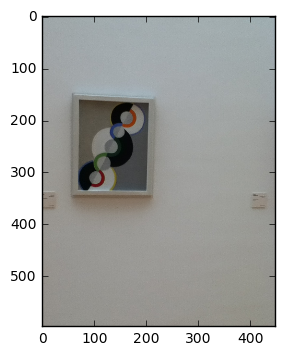
\includegraphics[width=\textwidth]{img/sample3_30P-0976.png}
\caption{Image with label 30P\label{fig:sample3_id}}
\end{subfigure}
\begin{subfigure}[b]{0.3\textwidth}
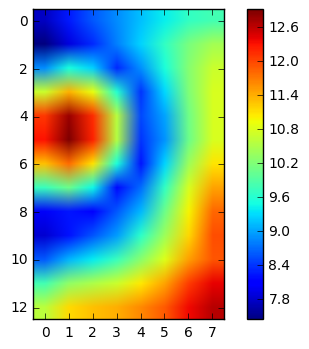
\includegraphics[width=\textwidth]{img/sample3_heatmap.png}
\caption{Heat-map for 30P\label{fig:sample3_hm}}
\end{subfigure}
\begin{subfigure}[b]{0.3\textwidth}
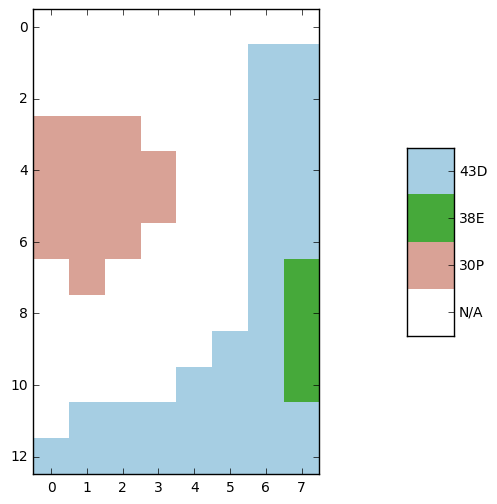
\includegraphics[width=\textwidth]{img/sample3_labels.png}
\caption{Label-map for 30P\label{fig:sample3_lab}}
\end{subfigure}
\caption{Sample images (scaled to a smaller side of 448 pixels)
along with the heat-map of maximal activation values
at each location when a fine-tuned ResNet-152 is applied to the image in a
strided manner, as well as the labels of all maximal activations that are
greater than the mean maximal activation\label{fig:heatmaps}}
\end{figure}

Figure~\ref{fig:heatmaps} shows images, along with the heat map
representing the maximal activation of a fine-tuned ResNet-152 at
each coordinate, when the network is applied in a strided manner
across the input image. The fine-tuning was carried out as described in
Section~\ref{sec:finetuning}.
From this image, we can see that the highest maximal
activations of the network usually occur at the location of the object.
This is true even if the object is not correctly classified by some of
the highest activations as can be seen in images
~\ref{fig:sample2_id}~-~\ref{fig:sample2_lab}.

In the images
~\ref{fig:sample3_id}~-~\ref{fig:sample3_lab}, it seems like many
high maximal activations occur specifically in the background area.
However, the corresponding label-map shows that these areas correspond
to the labels 38E and 43D. Both of these labels are pieces of art which
consist mostly of the background wall. In this sense, it is not
entirely wrong to consider 'wall-only' patches of the image as instances of
these pieces of art. This simply means that the image consists of two
separate regions of interest: one region with the painting (label 30P)
and one region with the wall (labels 38E/43D).

From these observations, we can confirm the assumption that the
maximal activations of a fine-tuned network are a good indicator of
the location of an object, or a combination of different objects.
Using this assumption, there is no need
for a procedure to annotate regions of interest, as employed by most
image retrieval approaches. % TODO

On the other hand, using datasets developed for image retrieval,
such as Paris6k or Oxford5k~\cite{philbin_lost_2008,philbin_object_2007},
this assumption cannot be applied, since the dataset is not clean
enough for a fine-tuned network to be a good indicator of location of
the query objects.

\subsection{Incorrectly identified images}\label{sec:incorrectimages}
\begin{figure}
\centering
\begin{subfigure}{\textwidth}
\begin{tabular}{|c|*{6}{c}}
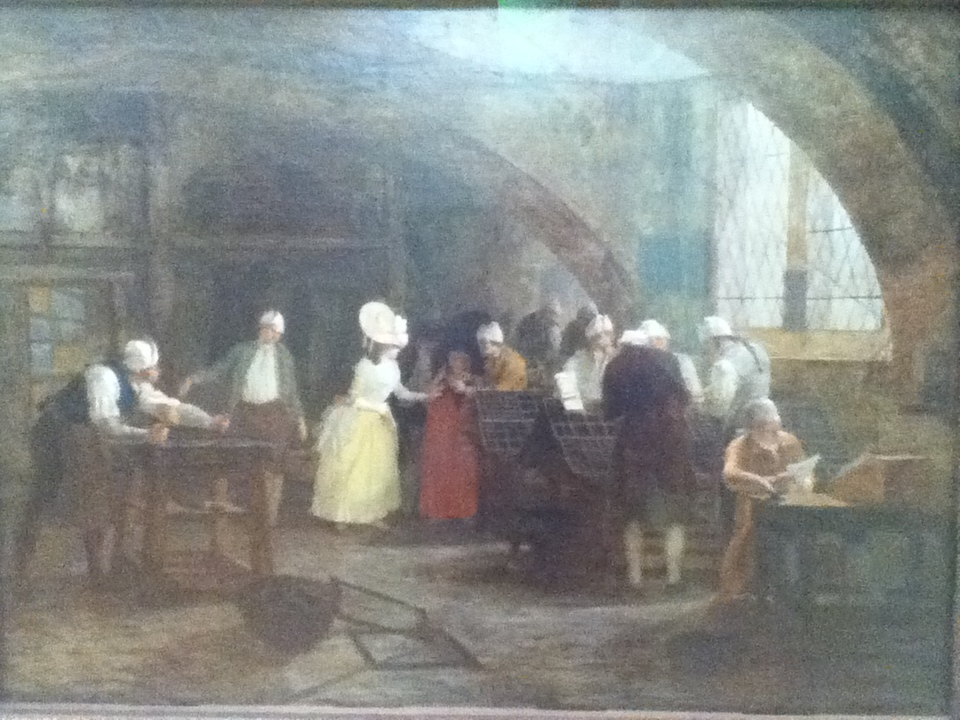
\includegraphics[width=0.12\textwidth]{img/11J-0521.JPG} &
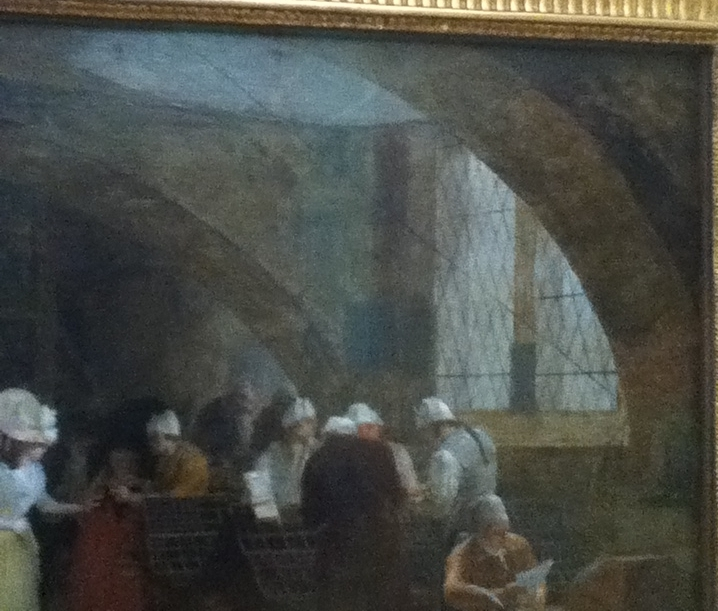
\includegraphics[width=0.12\textwidth]{img/11J-0.JPG} &
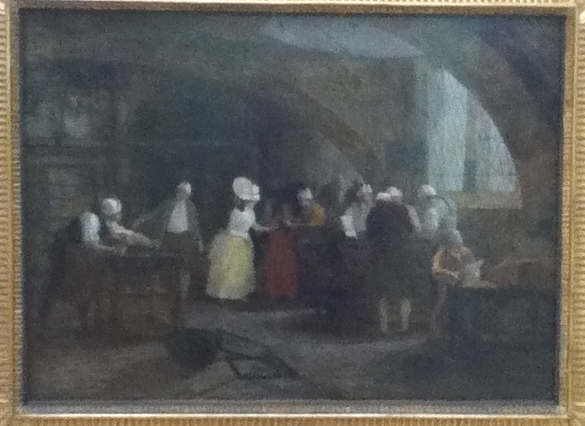
\includegraphics[width=0.12\textwidth]{img/11J-1.JPG} &
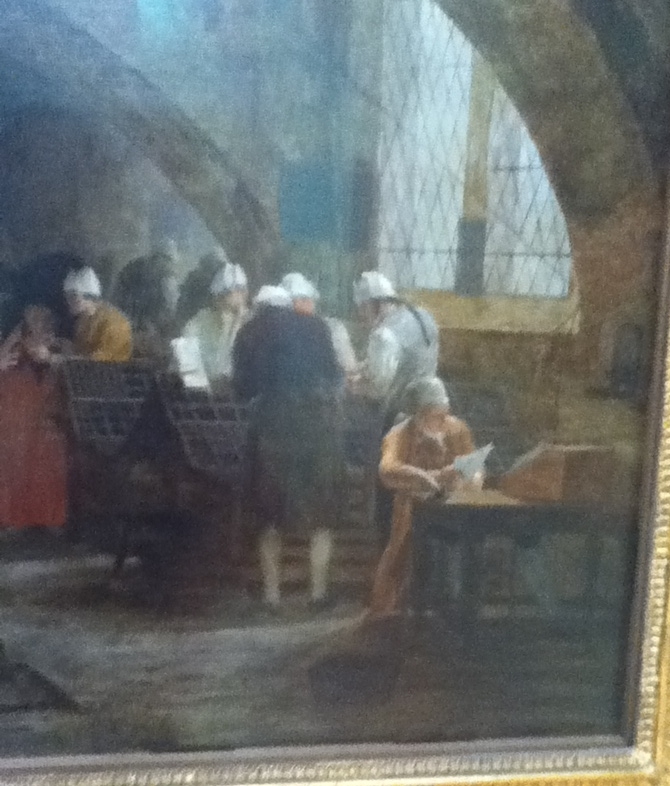
\includegraphics[width=0.12\textwidth]{img/11J-2.JPG} &
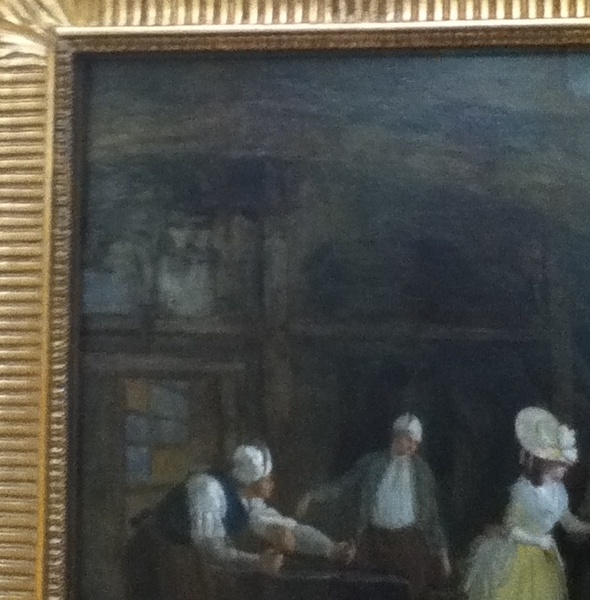
\includegraphics[width=0.12\textwidth]{img/11J-3.JPG} &
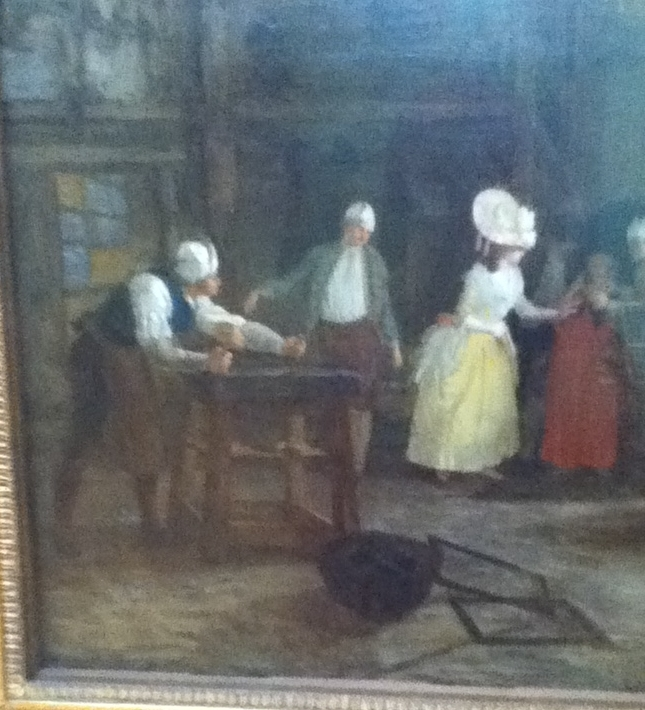
\includegraphics[width=0.12\textwidth]{img/11J-4.JPG} \\
\end{tabular}
\caption{Correctly identified query with label 11J,
along with its reference images.\newline
Average precision Gordo's net: 1.0, fine-tuned ResNet-152: 1.0
\label{fig:correct11J}}
\end{subfigure}

\begin{subfigure}{\textwidth}
\begin{tabular}{|c|*{6}{c}}
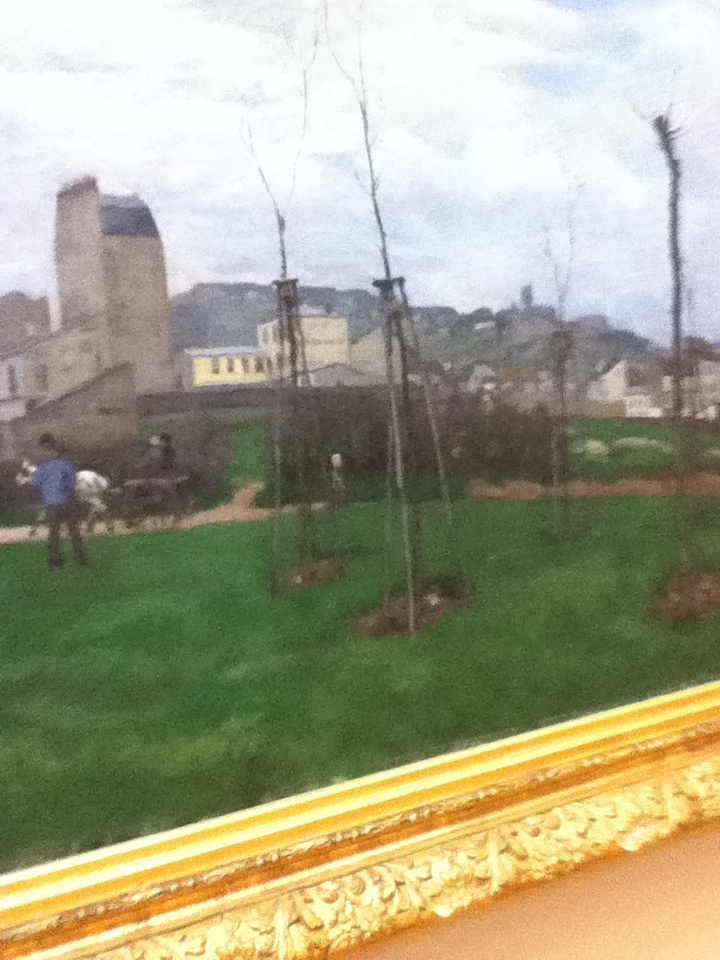
\includegraphics[width=0.12\textwidth]{img/23D-0740.JPG} &
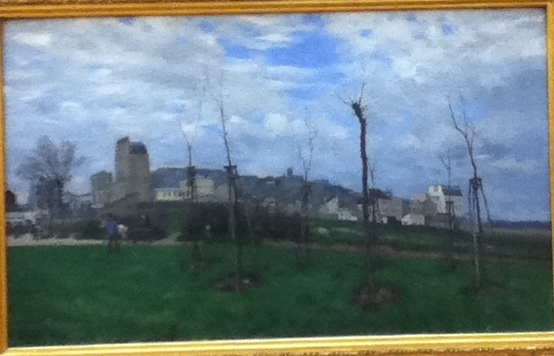
\includegraphics[width=0.12\textwidth]{img/23D-0.JPG} &
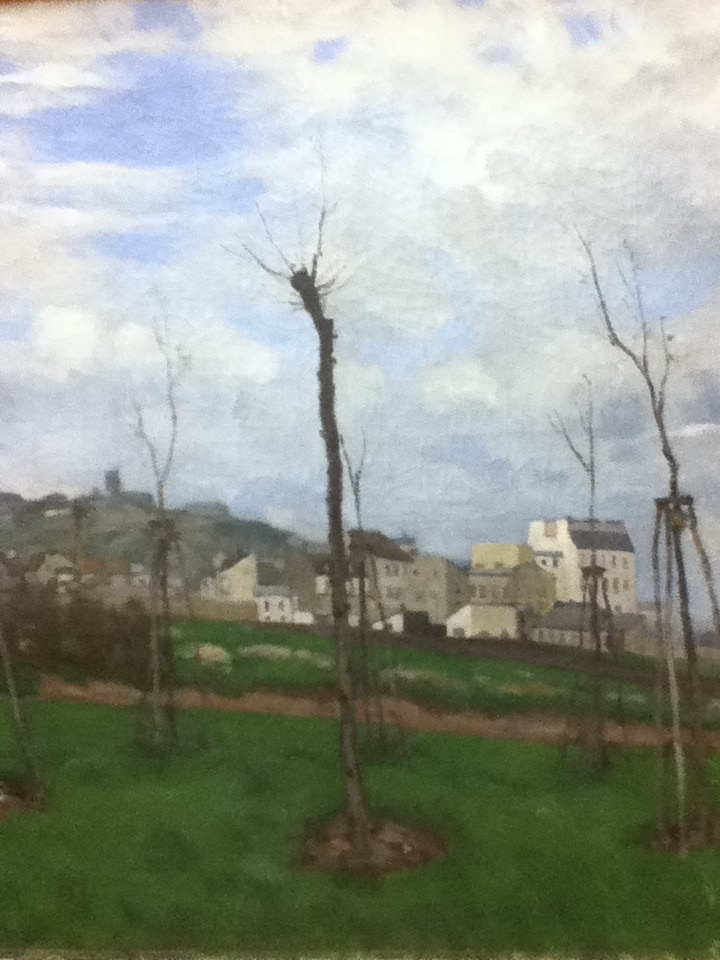
\includegraphics[width=0.12\textwidth]{img/23D-1.JPG} &
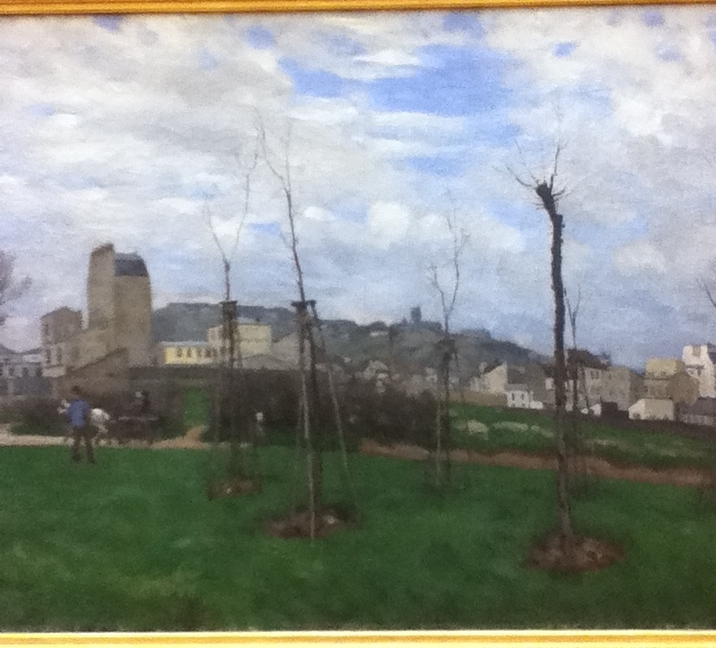
\includegraphics[width=0.12\textwidth]{img/23D-2.JPG} &
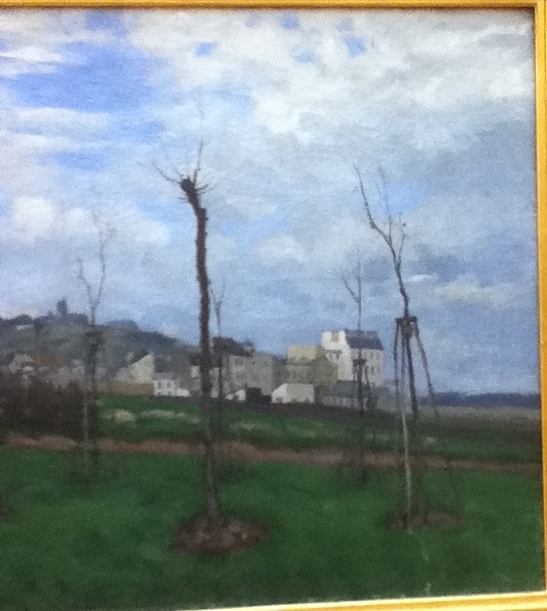
\includegraphics[width=0.12\textwidth]{img/23D-3.JPG} &
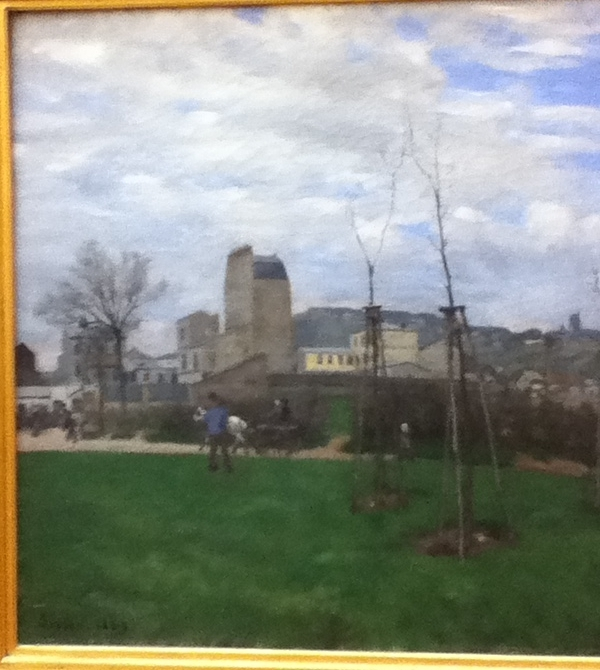
\includegraphics[width=0.12\textwidth]{img/23D-4.JPG} &
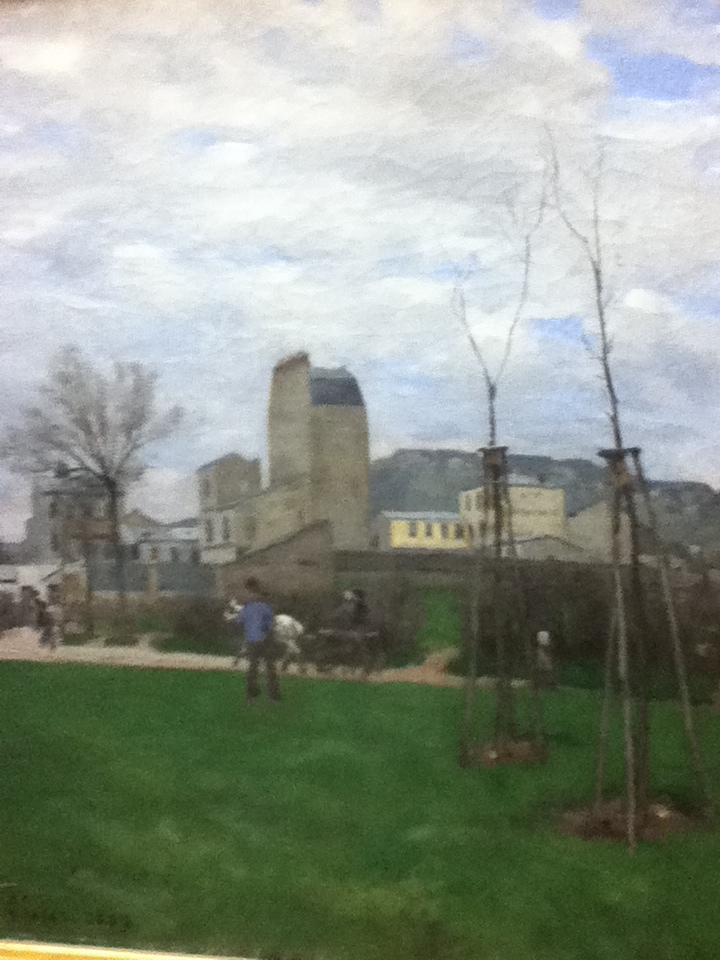
\includegraphics[width=0.12\textwidth]{img/23D-5.JPG} \\
\end{tabular}
\caption{Correctly identified query with label 23D,
along with its reference images.\newline
Average precision Gordo's net: 1.0, fine-tuned ResNet-152: 1.0
\label{fig:correct23D}}
\end{subfigure}

\begin{subfigure}{\textwidth}
\begin{tabular}{|c|*{6}{c}}
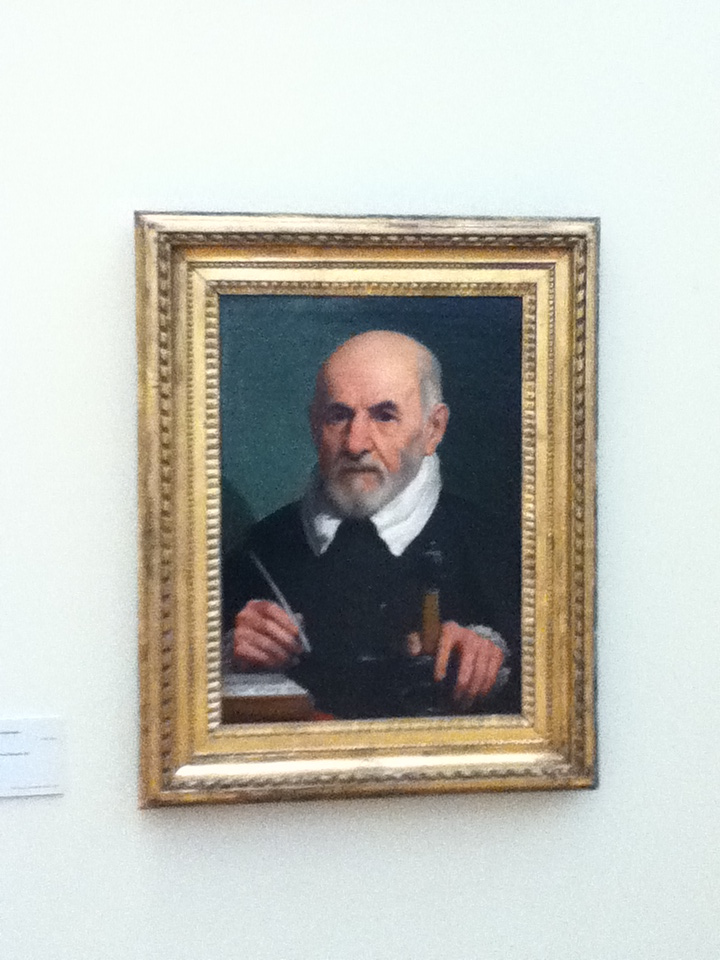
\includegraphics[width=0.12\textwidth]{img/1C-0454.JPG} &
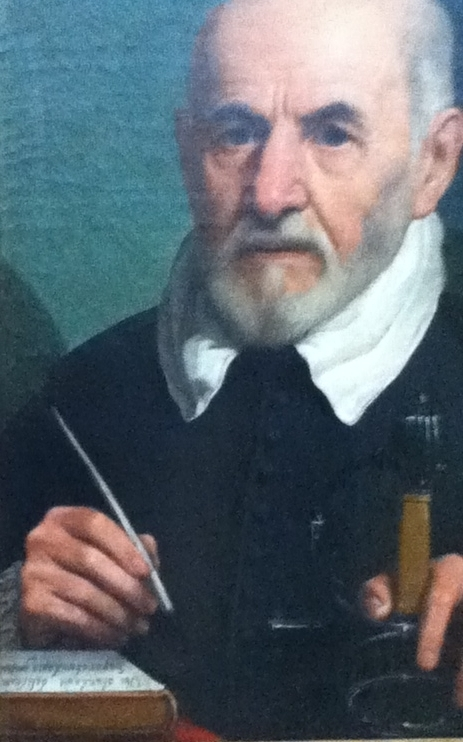
\includegraphics[width=0.12\textwidth]{img/1C-0.JPG} &
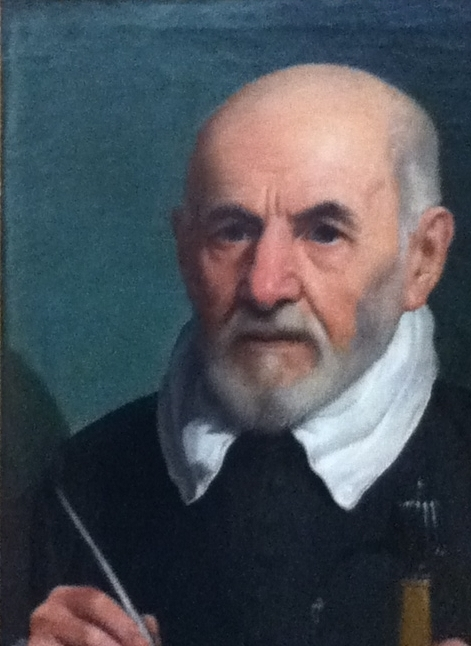
\includegraphics[width=0.12\textwidth]{img/1C-1.JPG} &
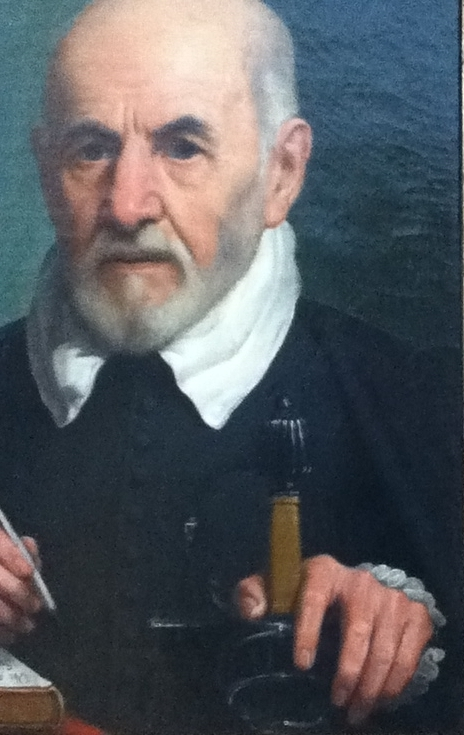
\includegraphics[width=0.12\textwidth]{img/1C-2.JPG} &
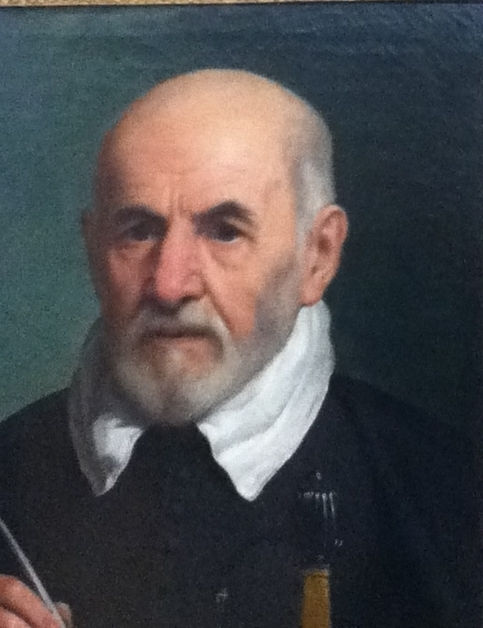
\includegraphics[width=0.12\textwidth]{img/1C-3.JPG} &
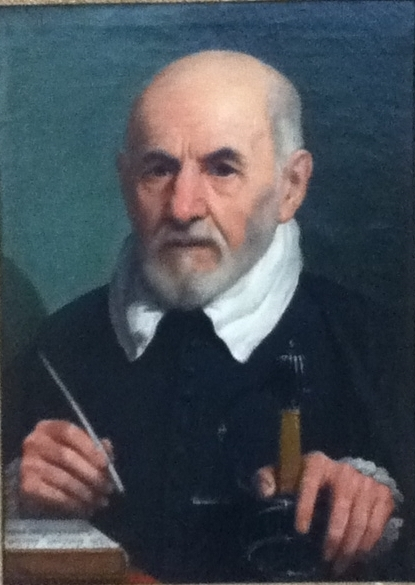
\includegraphics[width=0.12\textwidth]{img/1C-4.JPG} \\
\end{tabular}
\caption{Incorrectly identified query with label 1C,
along with its reference images.\newline
Average precision Gordo's net: 0.113, fine-tuned ResNet-152: 0.014
\label{fig:incorrect1C}}
\end{subfigure}

\begin{subfigure}{\textwidth}
\begin{tabular}{|c|*{6}{c}}
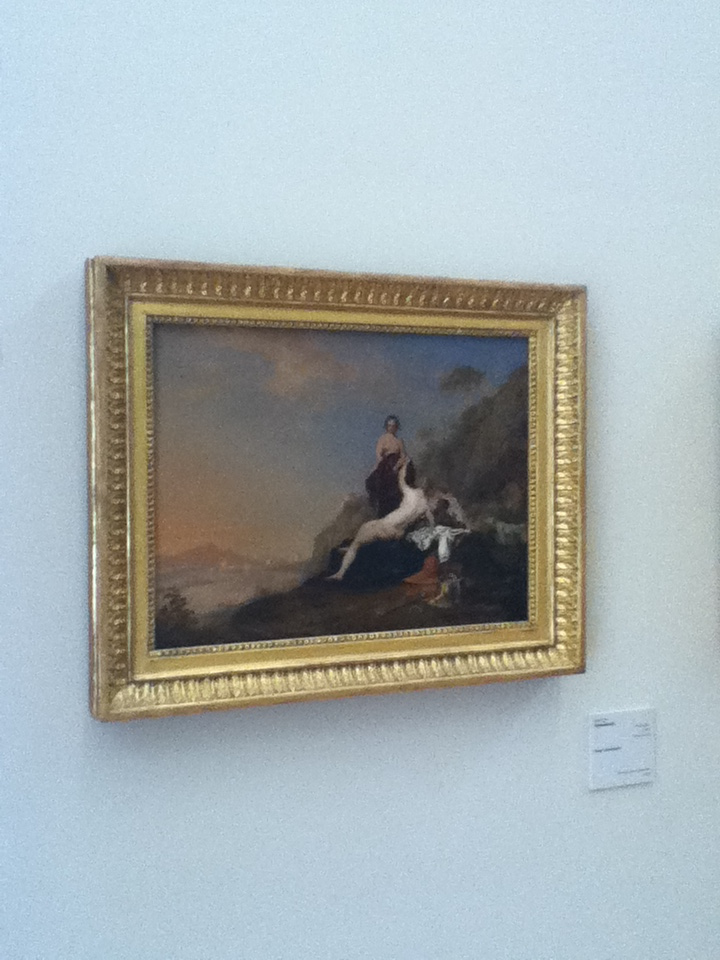
\includegraphics[width=0.12\textwidth]{img/5B-0506.JPG} &
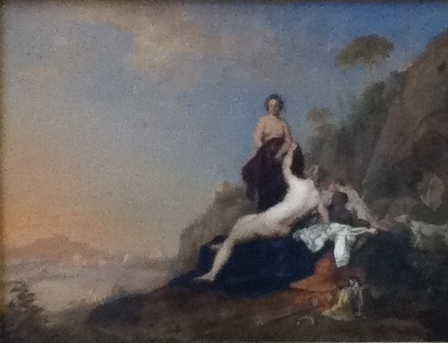
\includegraphics[width=0.12\textwidth]{img/5B-0.JPG} &
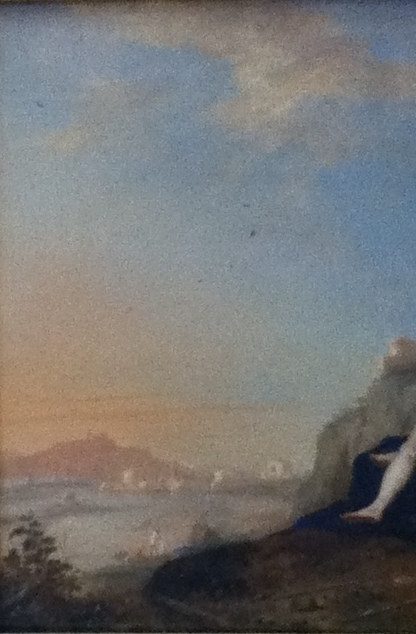
\includegraphics[width=0.12\textwidth]{img/5B-1.JPG} &
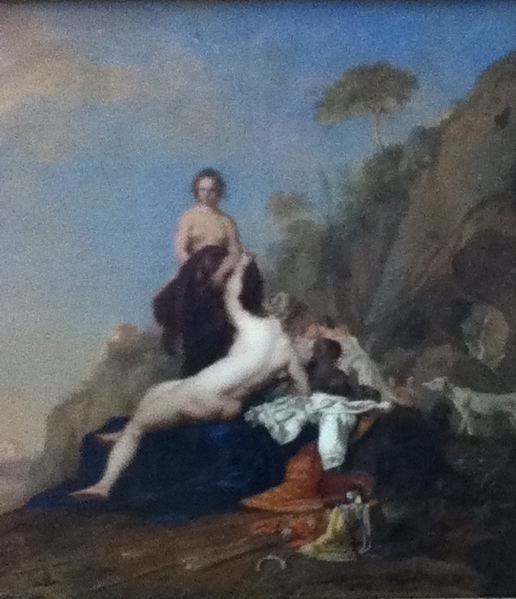
\includegraphics[width=0.12\textwidth]{img/5B-2.JPG} &
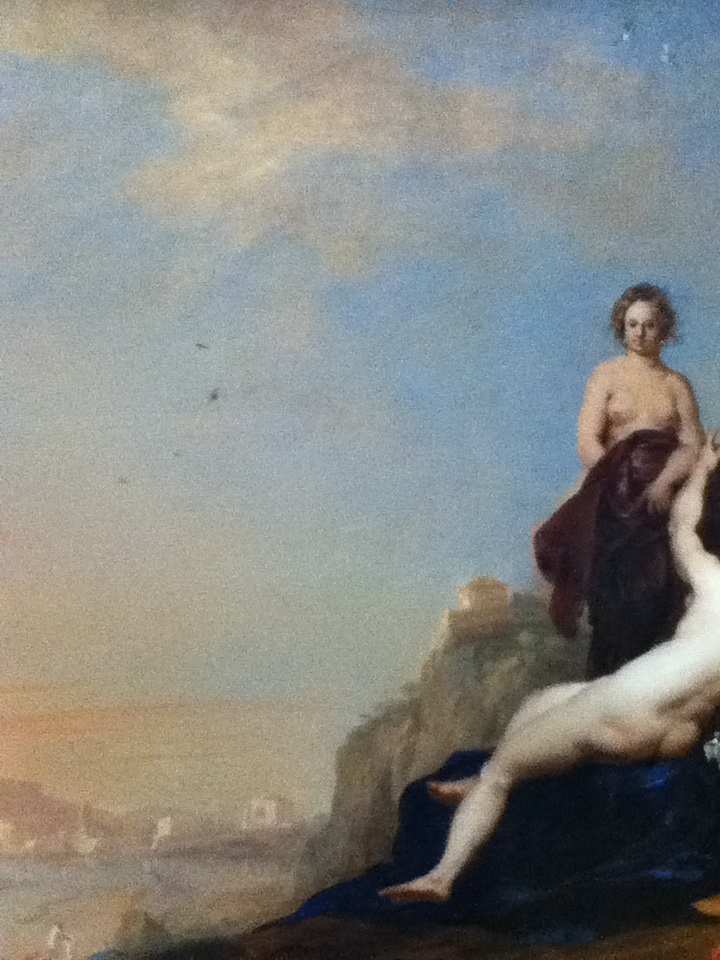
\includegraphics[width=0.12\textwidth]{img/5B-3.JPG} &
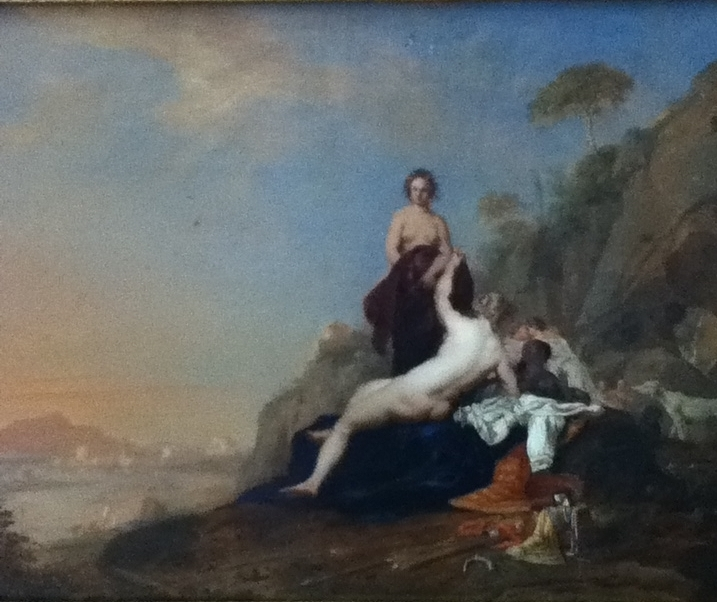
\includegraphics[width=0.12\textwidth]{img/5B-4.JPG} \\
\end{tabular}
\caption{Incorrectly identified query with label 5B,
along with its reference images.\newline
Average precision Gordo's net: 0.013, fine-tuned ResNet-152: 0.002
\label{fig:incorrect5B}}
\end{subfigure}

\begin{subfigure}{\textwidth}
\begin{tabular}{|c|*{6}{c}}
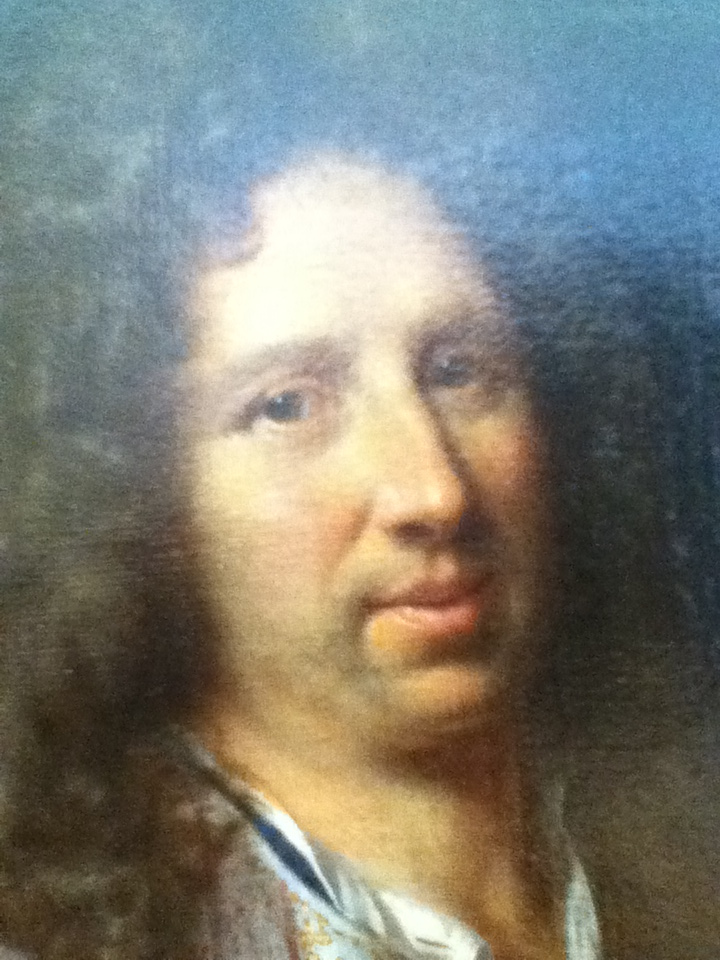
\includegraphics[width=0.12\textwidth]{img/11C-0351.JPG} &
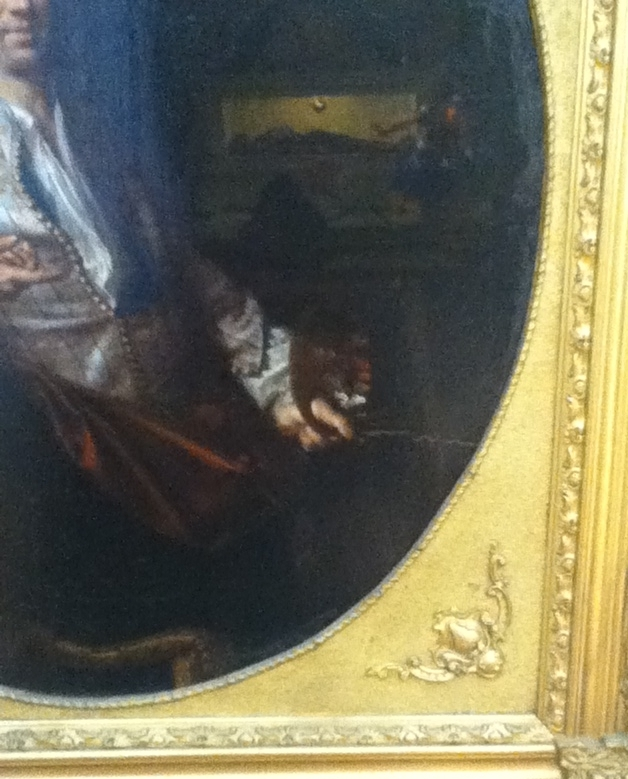
\includegraphics[width=0.12\textwidth]{img/11C-0.JPG} &
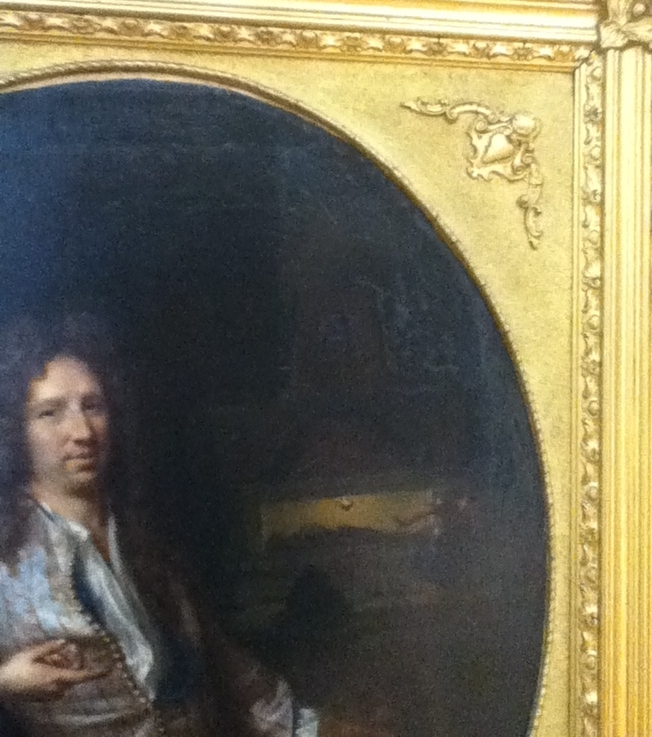
\includegraphics[width=0.12\textwidth]{img/11C-1.JPG} &
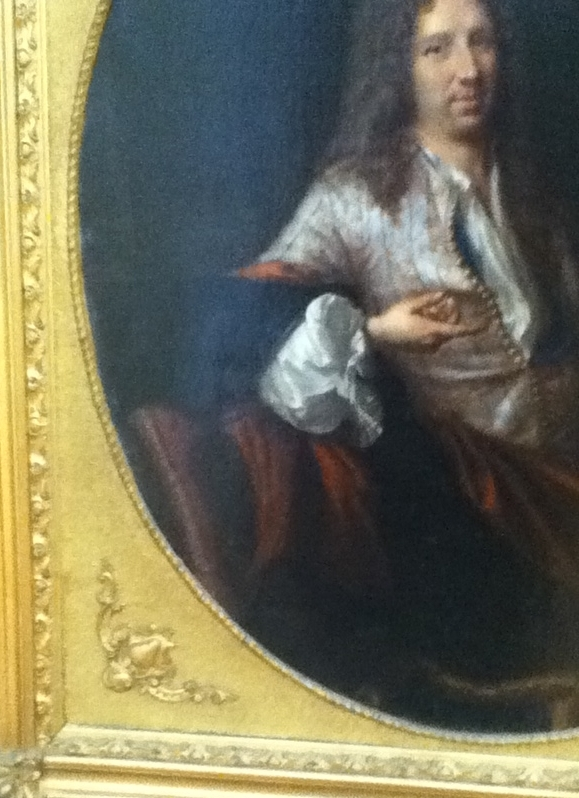
\includegraphics[width=0.12\textwidth]{img/11C-2.JPG} &
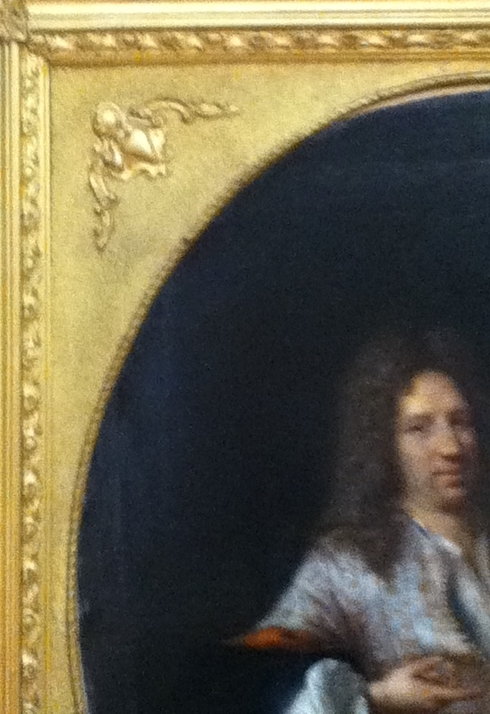
\includegraphics[width=0.12\textwidth]{img/11C-3.JPG} &
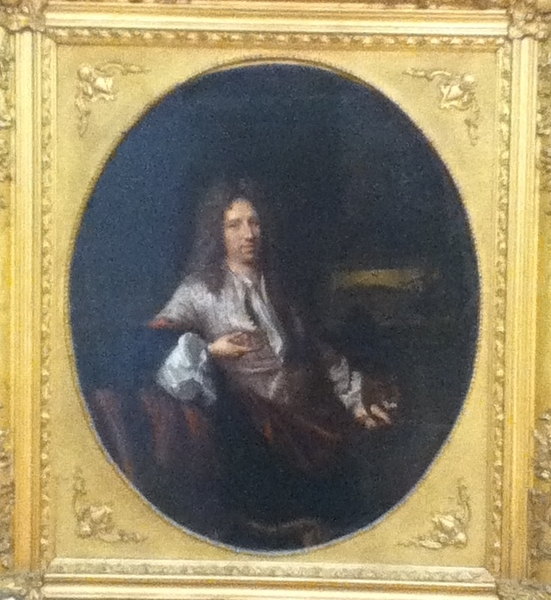
\includegraphics[width=0.12\textwidth]{img/11C-4.JPG} \\
\end{tabular}
\caption{Incorrectly identified query with label 11C,
along with its reference images.\newline
Average precision Gordo's net: 0.004, fine-tuned ResNet-152: 0.004
\label{fig:incorrect11C}}
\end{subfigure}
\caption{Sample images that were correctly and incorrectly identified
by a fine-tuned ResNet-152, as well as the network published by Gordo
et al.~\cite{gordo_deep_2016}, referred to as Gordo's net. For each image,
the query image is shown at the very left and all possible correct reference
images are shown to the right of the query. The caption contains the
associated average precision values.
\label{fig:incorrectimg}}
\end{figure}

Figure~\ref{fig:incorrectimg}
shows typical images that were correctly identified versus images that
were incorrectly identified, by a fine-tuned network as well as the network
published by Gordo et al.~\cite{gordo_deep_2016}, along with the average
precision for the respective queries.

From these results, we see that the networks struggle with images at
very different scales, achieving very low average precision,
while images with similar scales are usually perfectly matched.

% TODO more detail
Combining both of the properties identified in this section, we
propose a novel approach to learn a strong descriptor for instance
search in the next section.

\section{Proposed approach}\label{sec:proposed}
The proposed approach is based on multiple steps as described in the
following sections.

\subsection{Fine-tuning on classification using an FCN}\label{sec:fcnfinetune}
As shown in Section~\ref{sec:analysisprev}, a fine-tuned CNN is already
a good indicator of the location of an object in our datasets.
Additionally, it seems like scale is a particularly important factor.

Thus, the idea is to start by fine-tuning a network with images
at different scales. This can be achieved by using a fully
convolutional network (FCN), as introduced by
Long et al.~\cite{long_fully_2015}.

In a FCN, the final fully connected layers
of a network are replaced by convolutional layers having a kernel
which fits the entire domain of the output of the previous layer.
This type of convolution is equivalent to a fully connected layer,
but allows inputs (and outputs) of any size.
The effect is that the network can be applied in one pass to an
arbitrarily sized image. The output then represents the activations
of the network as if it was applied in a strided manner across the image.
The stride of a full network depends on the architecture and is 32
pixels for the architectures used here: AlexNet and ResNet.

Once a FCN is applied to the image, the loss
is calculated by averaging the cross-entropy loss across all locations
and outputs.
The final loss is then obtained by passing images at different scales
through the FCN and averaging across all cross-entropy losses of all
outputs and scales. Equation~\ref{eq:fcnloss} shows the loss for a
single image. $S$ represents the number of scales at which the image
is passed through the network.
$H_s$ and $W_s$ represent the height and width of the feature
map respectively, given the scale $s$ of the input image. $y^{h,w}$
represents the prediction of the network at spatial location
$(h,w)$ in the full feature map.

\begin{equation}\label{eq:fcnloss}
\mathcal{L} = \frac{1}{S} \sum_{s=1}^S - \frac{1}{H_s*W_s}
\sum_{h=1}^{H_s} \sum_{w=1}^{W_s} y^{h,w} \log \hat{y} +
(1-y^{h,w}) \log (1-\hat{y})
\end{equation}

We can see from the Equation that we chose to give each scale of the image
the same weight in the loss. Additionally, we can see that this loss can
only be applied to one image at a time, hence the true label $\hat{y}$ is
a constant in Equation~\ref{eq:fcnloss}.
This is because the images are passed to the network at their true
aspect ratio, which means the loss for different images may have different
values for the heights and widths of the feature maps $H_s$ and $W_s$.

In order to normalize the sizes of the features present in the images,
all images are scaled to have the same
number of pixels in the smaller side. Note that for large aspect
ratios and large scales of the smaller side,
the memory consumption of training can be high for single images
having a very large aspect ratio. To limit this spike in memory
consumption, the aspect ratios are limited by introducing uniform
random noise on the smaller side of images with high aspect ratios.

In our experiments, we use a maximal aspect ratio of $2.0$ and images
at two scales of $448$ and $224$ pixels for the smaller side. We found
that the AlexNet architecture did not have good convergence behavior,
thus we used scales of $384$ and $224$ instead.

\subsubsection{Gradient descent using micro-batches}
Since only a single image is passed to the network at a time, the
stochastic gradient descent algorithm used to optimize the parameters
of the model does not converge, as a single image is not representative
of the dataset as a whole and does not form a large enough mini-batch.

Instead, we form a mini-batch by accumulating gradients from many
\emph{micro-batches}, each of which is made up of only a single image.
This allows to form a mini-batch of any size to obtain stable convergence
in stochastic gradient descent.

However, using a micro-batch formed of a single image represents an issue
with the ResNet architecture: this model uses batch-norm layers, introduced
by Ioffe et al.~\cite{ioffe_batch_2015}. When training a model, the layer
normalizes each batch by its mean and variance. However, it keeps a running
mean and variance, which approximates the true mean and variance of the
dataset and which is applied during testing. With a micro-batch size
of 1, this running mean and variance cannot be inferred, which leads to
very poor behavior of the model. Instead, we pre-train the model on the
dataset as described in Section~\ref{sec:finetuning} in order to obtain
a correct estimate of the running mean and variance. Then, we preset the
network with the parameters of this fine-tuned network when training the
FCN as described above.

\subsection{Descriptor extraction network}
\begin{figure}
\begin{subfigure}{\textwidth}
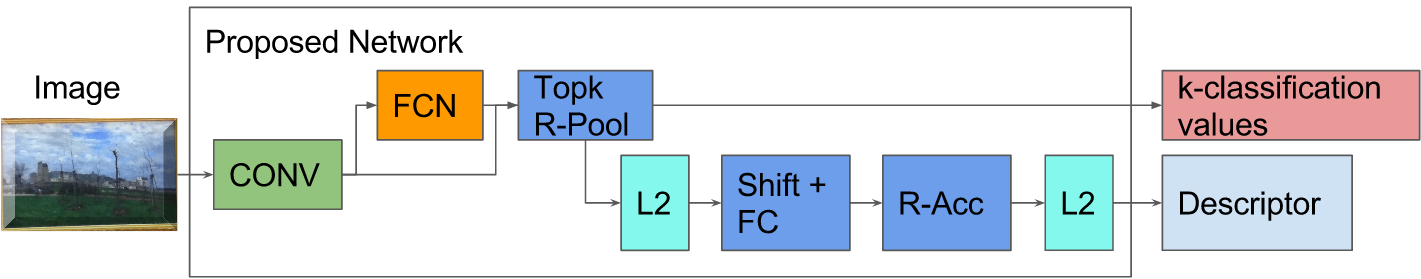
\includegraphics[width=\textwidth]{img/contrib_deploy.png}
\caption{Proposed architecture for instance search, at deploy time
\label{fig:contribdeploy}}
\end{subfigure}

\begin{subfigure}{\textwidth}
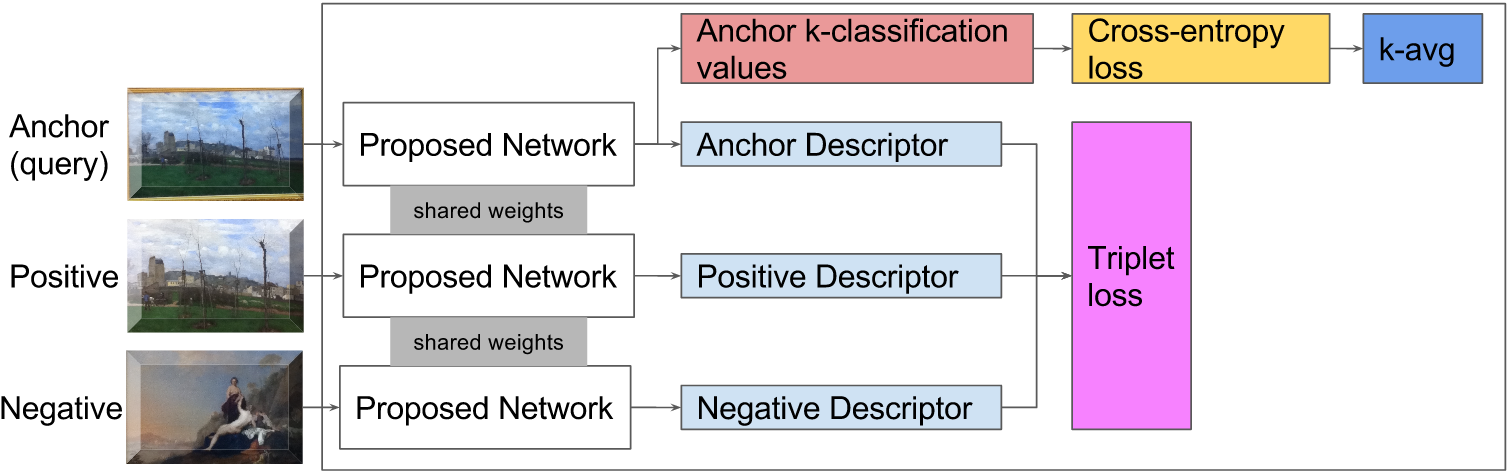
\includegraphics[width=\textwidth]{img/contrib_train.png}
\caption{Proposed architecture for instance search, at training time
\label{fig:contribtrain}}
\end{subfigure}
\caption{Proposed architecture for instance search, based on a FCN
~\cite{long_fully_2015} for region proposals. The descriptor extraction
for each region is similar to the architecture by
Gordo et al.~\cite{gordo_deep_2016}, as shown in
Figures~\ref{fig:gordo_deploy}~and~\ref{fig:gordo_train}
\label{fig:contrib}}
\end{figure}

The second step of the proposed approach relies on the FCN, trained
as described in the first step in Section~\ref{sec:fcnfinetune}.

Figure~\ref{fig:contrib} illustrates the proposed architecture.
To obtain a descriptor, we first apply the convolutional layers of
a previous architecture, such as AlexNet or ResNet. We then obtain all
classification outputs at all locations using the pre-trained FCN.
We only consider the maximal activation at all locations.
The locations with the top $k$ maximal activations will form the descriptor.

For each of these locations, we closely follow the architecture
proposed by Gordo et al.~\cite{gordo_deep_2016}, as shown in
Figure~\ref{fig:gordo_deploy}. The convolutional features are
reduced by a $\|\cdot\|_2$-normalization, then a shifting and fully connected
layer. Finally, all descriptors from the $k$ locations are
sum-aggregated and $\|\cdot\|_2$-normalized again.

When training, the network is applied to a triplet of images.
These triplets are chosen as described in Section~\ref{sec:simplifiedsiam}
for the simplified Siamese architecture.

Additionally, we regularize the triplet loss by a cross-entropy loss
to make sure that the $k$ locations with highest
maximal activations are correctly classified. This loss is averaged over
the $k$ locations.

Equation~\ref{eq:proposedloss} shows the full loss as used in our
experiments to train the proposed model, for a $N$ images. In this
equation, $(h_l, w_l)$ represent the spatial coordinates of the $l$-th
region of highest maximal activation in the feature map produced by
the FCN.

\begin{equation}\label{eq:proposedloss}
\mathcal{L} = \sum_{i=1}^N \left( \max(0, x^a_i x^n_i - x^a_i x^p_i + m) +
\alpha \frac{1}{N} \frac{1}{k} \sum_{l=1}^k -
y_i^{h_l,h_l} \log \hat{y}_i + (1-y_i^{h_l,w_l}) \log (1-\hat{y}_i) \right)
\end{equation}

In our experiments, we choose the number of regions with highest maximal
activation to be $k=4$ and the regularization hyper-parameter $\alpha=1.0$.
The margin of the triplet loss is $m=0.1$ as described in
Section~\ref{sec:simplifiedsiam}.

\subsection{Advantages}
As shown in Section~\ref{sec:analysisprev}, this approach
allows the network to decide which region of interest is
best suited for classification and ultimately which regions
are best suited for comparison with other images.

Another advantage is that this approach does not require
any annotation of the images with regions of interest,
which can be a long, manual or automatic process, as evident
from the cleaning process used by Gordo et al.~\cite{gordo_end--end_2016}.

Finally, an important property of the descriptor is that it
heavily relies on the classification
capabilities of the network. This means the descriptor is
mostly meaningless for a different dataset and needs
to be learned for each dataset. This can be an advantage,
since the descriptor can be better suited to a particular
dataset and the learning process does not take long, as shown
in Section~\ref{sec:perfresults}. On the other hand, this means that
the descriptor cannot be applied in a typical image retrieval
task.

% !TeX root = ../full_report.tex

\chapter{Evaluation}\label{sec:evaluation}
\section{Datasets}\label{sec:datasets}
The proposed approaches as well as several base-lines are evaluated
on two datasets: the CLICIDE and GaRoFou datasets. These datasets are
described in detail by Portaz et al.~\cite{portaz_construction_2017}.
Both datasets are typical of instance search datasets
in museums or touristic sites: the objects represented by their images
are paintings for one and glass cabinets containing sculptures and artifacts
for the other dataset. Both datasets contain a small number of images
per instance and a small number of images in total.
Table~\ref{tab:datasets} lists the content and statistics of the datasets
in detail. In particular, this table shows that the total number of images
is quite small (order of magnitude of 1000), the number of instances
is large both in the dataset as well as the test sets (order of magnitude
of 100), and the median number of images per instance is small
(2 for GaRoFou, 6 for CLICIDE). This sets both datasets clearly apart
from the most common datasets used in image retrieval, such as
Oxford~\cite{philbin_object_2007}, Paris~\cite{philbin_lost_2008}
as well as Holidays~\cite{jegou_hamming_2008}.

\begin{table}
\begin{tabular}{|l|l|l|}
\hline & \emph{CLICIDE} & \emph{GaRoFou}\\
\hline \emph{Type of objects} & Paintings & Glass cabinets
containing various objects\\
\hline \emph{\#Instances} & 464 & 311\\
\hline \emph{\#Reference images} & 3245 & 1068\\
\hline \emph{\#Query images (\#instances)} & 165 (134) & 184 (166)\\
\hline \emph{Median \#images per instance} & 6 & 2\\
\hline \emph{Min \#images per instance} & 1 & 1\\
\hline \emph{Max \#images per instance} & 22 & 45\\
\hline \emph{Total reference images (\#instances)} & 3452 (473) & 1068 (311)\\
\hline \emph{Total query images (\#instances)} & 177 (143) & 184 (166)\\
\hline
\end{tabular}
\caption{Details of the datasets used for evaluation\label{tab:datasets}}
\end{table}

\subsection{CLICIDE}
The CLICIDE dataset contains photographs taken in the Grenoble Museum of Art.
The objects represented in the photographs are paintings and still images,
exclusively. The full dataset contains 207 images with no meaningful content,
mostly showing walls. These images are labeled as such and have been filtered
from the dataset in our evaluation. This explains the difference between
total number of images and number of images in Table~\ref{tab:datasets}.
Furthermore, there are 12 query images which contain objects not
present in the reference images. These have been filtered out as well.

The CLICIDE dataset is characteristic because the different images
for each instance usually consist of at least one global view of the
painting and multiple other images representing sub-regions of the
same painting.

\subsection{GaRoFou}
The GaRoFou dataset contains high-resolution photographs taken in the
Museun of Fourvière in Lyon. The objects represented in the photographs
are a cultural heritage collection: sculptures, steles and small artifacts
grouped together in glass cabinets.

The full GaRoFou dataset is larger than the part used here: along with
the dataset of images, it contains a dataset of videos as well as images
extracted from these videos. The video collection has not been used as
part of our research.

\section{Metrics}
There are several commonly used metrics in classification and information
retrieval. The following sections define these metrics and their use
in our research.

\subsection{Precision}\label{sec:precision}
\begin{equation}\label{eq:preccls}
P = \frac{TP}{PRED}
\end{equation}

\begin{equation}\label{eq:precir}
P_q = \frac{RR_q}{RET}
\end{equation}

\begin{equation}\label{eq:preck}
P_q@k = \frac{RR^k_q}{k}
\end{equation}

\begin{equation}\label{eq:prec1}
MP@1 = \frac{1}{Q} \sum_q P_q@1
\end{equation}

In classification, precision is a measure of how many correct predictions
were made out of all predictions. Equation~\ref{eq:preccls} shows this
relationship: $TP$ are the true positives, the correct predictions,
and $PRED$ is the number of all predictions, including incorrect ones.
$PRED$ is usually equal to the size of the testing dataset in classification.

In information retrieval, similarly,
precision and more generally precision$@k$ is a measure of how many
relevant documents were retrieved out of all retrieved documents.
However, the metric is evaluated for each query, instead of the whole
testing dataset.
Equations~\ref{eq:precir}~and~\ref{eq:preck} illustrate this: $P_q$ is
the precision for query $q$, $RR_q$ represents the number of retrieved
and relevant documents for query $q$.
$RET$ represents the total number of retrieved documents. Finally, $RR^k_q$
represents the number of retrieved, relevant documents out of the $k$ first
retrieved documents for query $q$.

Thus, precision$@k$ simply uses a cut-off at $k$: it measures how many
relevant documents there are in the first $k$ retrieved documents.

In instance search, only the first retrieved document is important:
If the first result is correct, we correctly identify the instance.
Hence, we are mostly interested in the precision@1 metric here.
In order to generalize this metric to all queries, the mean precision@1
is used, as defined in Equation~\ref{eq:prec1}. In this equation,
$Q$ represents the number of queries.

\subsection{Mean average precision}
\begin{equation}\label{eq:recall}
R_q = \frac{RR_q}{REL_q}
\end{equation}

\begin{equation}\label{eq:ap}
AP_q = \frac{1}{REL_q} \sum_{k=1}^{RET} rel(RET_k)P@k
\end{equation}

\begin{equation}\label{eq:map}
MAP = \frac{1}{Q} \sum_q AP_q
\end{equation}

In information retrieval, average precision is commonly used, since it
allows to consider the order in which documents are returned by a system.
Average precision represents the area under the precision-recall curve
for a given query $q$. Recall for query $q$ is defined as in
Equation~\ref{eq:recall} as the fraction of retrieved, relevant documents
for query $q$ as compared to all relevant documents to query $q$.

Equation~\ref{eq:ap} defines average precision for a given query $q$:
it can be expressed as a finite sum
over the precision@k values at every possible cut-off $k$, multiplied by an
indicator $rel(RET_k)$, which is 1 if the $k$-th retrieved document is
relevant. This sum is then normalized by the total number of relevant
documents for query $q$ $REL_q$.
Note that in the literature, different definitions of average precision can
be found. We chose to follow a common definition of this metric, which
is shared by the Oxford~\cite{philbin_object_2007} and the
Paris~\cite{philbin_lost_2008} datasets.

Finally, mean average precision $MAP$ represents the mean of all average
precision values over $Q$ queries, as defined in Equation~\ref{eq:map}.

In instance search, mean average precision is not as important as in image retrieval,
since we only care about the first ranked result. Nevertheless, it can be an interesting
metric to allow better comparison between different systems, so we compute
the mean average precision for all results along with the mean precision@1.

\section{Evaluation methodology}\label{sec:evalmethod}
Unless explicitly noted, an evaluation of the system is carried out as
follows:

All reference images are encoded with a descriptor extracted from the
network to be tested. The query image is encoded the same way.
All descriptors are normalized and the descriptor of the query image
is compared to all reference images by computing the dot product between
it and all descriptors of the reference images. This can be performed
by a single vector-matrix multiplication. The resulting values describe
the cosine similarity between the descriptor of the query image
and the descriptors of reference images.

This is because the cosine similarity between two normalized vectors is
equal to the dot product between the two vectors, from the definition
of the cosine similarity. Furthermore, Equation~\ref{eq:sqdistcosdot} shows
that the dot product is closely related to the squared
euclidean distance between two normalized vectors.
This means that a high cosine similarity, high value of the dot product
and low squared euclidean distance between two descriptors have the
same meaning in the context of this research.

Hence, after a query image is compared to all reference images through
a vector-matrix multiplication, the index of the highest value in the
resulting vector indicates the most similar reference image.

\section{Baselines}\label{sec:baselines}
Table~\ref{tab:baselines} shows the baselines set for the two evaluation
datasets, as described in Section~\ref{sec:datasets}. The metric used
to compare systems is mean precision@1, as described in
Section~\ref{sec:precision}, and the evaluation is carried out as
described in Section~\ref{sec:evalmethod}.

\begin{table}
\begin{tabular}{|l|c|c|}
\hline & \emph{CLICIDE} & \emph{GaRoFou}\\
\hline \emph{SIFT} & 70.08 & 78.82\\
\hline \emph{AlexNet IN} & 72.73 & 85.87\\
\hline \emph{ResNet-152 IN} & 72.12 & 85.33\\
\hline \emph{Gordo et al.}~\cite{gordo_deep_2016} (ResNet-50) & 90.30 & \textbf{95.65}\\
\hline \emph{Gordo et al.}~\cite{gordo_deep_2016} (ResNet-50, multi-res)
& \textbf{92.73} & \textbf{95.65}\\
\hline
\end{tabular}
\caption{Evaluation base-lines set for the CLICIDE and GaRoFou datasets.
The results are expressed in percentage points of
mean precision@1\label{tab:baselines}}
\end{table}

The descriptors used for comparing images are extracted using different
methods.
The SIFT method has been previously evaluated by
Portaz et al.~\cite{portaz_construction_2017}, who have detailed this
evaluation.

For the \emph{AlexNet IN} and \emph{ResNet-152 IN} methods,
an AlexNet and ResNet-152 architecture is pre-trained on the ImageNet dataset.
Then, the descriptor is simply extracted by passing an image through the
convolutional layers of the
network and normalizing the output. For the ResNet architecture, the final
average pooling is performed as well to produce a descriptor of similar
dimensions to the others. This means the descriptor has dimension 2048
for the ResNet architecture and 9216 for the AlexNet architecture.

For all networks presented here which require images of a specific size,
all images are simply pre-processed by resizing them to the expected
size. Since the networks are based on networks built for the ImageNet
challenge
~\cite{russakovsky_imagenet_2015,he_deep_2016,krizhevsky_imagenet_2012},
the expected size is $224 \times 224$. The results of pre-trained
networks on ImageNet (\emph{AlexNet IN} and \emph{ResNet-152 IN}),
fine-tuned networks on classification (Section~\ref{sec:finetuning}) and
simplified Siamese networks (Section~\ref{sec:simplifiedsiam}) all use
images resized to $224 \times 224$.

The method by Gordo et al.~\cite{gordo_deep_2016}
is based on the pre-trained network published publicly, based on a ResNet-50
architecture. For this network, images are only pre-processed to have a
common size of 800 pixels on the smaller side of the image,
as the network works with region proposals and thus accepts
any scale of image. This network outputs a descriptor with 2048 dimensions.
Finally, the multi-resolution method uses input images with different
sizes of the smaller side (550, 800 and 1050 pixels).

\section{Performance}
The performance evaluation is carried out on a typical system used for
training CNNs.
The components approximately represent the highest standard available for a
single-GPU server architecture in 2016.

The server contains the following components:
\begin{enumerate}
    \item CPU: Intel\textsuperscript{\textregistered} Xeon\textsuperscript{\textregistered}
    E5-2623 v4, 16 cores, 10MB cache, 2.60GHz
    \item Memory: 144 GB, DDR4 % TODO mem speed
    \item Graphics card: NVIDIA\textsuperscript{\textregistered} Titan X, Pascal architecture,
    12 GB memory (two of such graphics cards were available but only one
    was used in the performance evaluation at a time)
\end{enumerate}

Performance is measured in time in milliseconds or hours required to
execute the task, as well as GPU memory required.
If multiple sub-tasks are performed for
a task, the reported performance is simply the accumulation of time and
the maximum of required GPU memory of the sub-tasks.
\subsection{Training}
The training performance is evaluated using the server as described above
and the CLICIDE dataset as described in Section~\ref{sec:datasets},
containing 3245 images.

The training performance was measured only for tasks specific to the dataset,
as other tasks can be performed once upfront for any dataset and parameter
weights can be transferred in a negligible amount of time.
In particular, this means
that pre-training a network on a dataset not specific to our task is
counted as using no time or memory.

\subsection{Testing}
The testing performance is evaluated using the server as described above and
the validation dataset of CLICIDE, as described in Section~\ref{sec:datasets}.
This dataset contains 165 images. However, the performance is reported
as the average performance for a single image, as this is the most common
use-case when applying the instance search system.

% !TeX root = ../full_report.tex

\chapter{Results}
In this section, we present the experimental results obtained in our
research.

\section{Performance}\label{sec:perfresults}

\begin{table}
\begin{tabular}{|l|c|c|}
\hline & \multicolumn{2}{c|}{\emph{CLICIDE training}}\\
\hline & Time (h) & GPU memory (MiB)\\
\hline \emph{AlexNet IN} & 0 & 0\\
\hline \emph{ResNet-152 IN} & 0 & 0\\
\hline \emph{Gordo et al.~\cite{gordo_deep_2016}} & 0 & 0\\
\hline \emph{Gordo et al.~\cite{gordo_deep_2016} (multi-resolution)}
& 0 & 0\\
\hline \emph{AlexNet FT} & 1.429 & 1706\\
\hline \emph{ResNet-152 FT} & 1.621 & 6910\\
\hline \emph{Proposed AlexNet} & 49.06 & 1956\\
\hline \emph{Proposed ResNet-152} & 86.62 & 10494\\
\hline
\end{tabular}
\caption{Performance of different approaches in terms of time in seconds and
maximal GPU memory usage in MB when training on the CLICIDE dataset
\label{tab:perftrain}}
\end{table}

Table~\ref{tab:perftrain} shows the performance of various approaches
when training on the CLICIDE dataset. We assume that pre-trained
networks have 0 cost. This table shows that fine-tuning a network
on classification on the new dataset is quite fast and has a low memory
footprint. This is interesting since fine-tuning already achieves better
results than many standard approaches, as can be seen in
Section~\ref{sec:evalresults}.
We can also see that training our proposed architecture is much
more costly, although the absolute cost is not excessive:
around 86h of training time in total for the very deep ResNet-152
and 49h for AlexNet, using our larger dataset with over 3000 images.

\begin{table}
\begin{tabular}{|l|c|c|}
\hline & \multicolumn{2}{c|}{\emph{CLICIDE test per image}}\\
\hline & Time (ms) & GPU memory (MiB)\\
\hline \emph{AlexNet IN} & 1.14 & 850\\
\hline \emph{ResNet-152 IN} & 23.9 & 972\\
\hline \emph{Gordo et al.~\cite{gordo_deep_2016}} & 200 & N/A\\
\hline \emph{Gordo et al.~\cite{gordo_deep_2016} (multi-resolution)}
& 900 & N/A\\
\hline \emph{AlexNet FT} & 4.6 & 1012\\
\hline \emph{ResNet-152 FT} & 26.1 & 944\\
\hline \emph{Proposed AlexNet} & 12.3 & 1116\\
\hline \emph{Proposed ResNet-152} & 45.2 & 2212\\
\hline
\end{tabular}
\caption{Performance of different approaches in terms of time in seconds and
maximal GPU memory usage in MB when testing on a single image
of the CLICIDE dataset\label{tab:perftest}}
\end{table}

Table~\ref{tab:perftest} shows the performance of the different networks
when evaluating on a single image. For the baseline based on SIFT, no performance measures were available.
For the Gordo et al.~\cite{gordo_deep_2016} baseline, we simply took the
measurements from their paper, performed on a slightly different system,
as we only have a slower version of the model available, which does not
evaluate the entire system on GPU, and is thus about 10 times slower.

We can see from Table~\ref{tab:perftest} that all networks
of the same architecture have approximately the same performance, with
the proposed architecture being 2-3 times slower than a network
fine-tuned on classification. However, compared to the best performing
network proposed by Gordo et al.~\cite{gordo_deep_2016}, the proposed AlexNet
is two orders of magnitude faster and the proposed ResNet152 is one
order of magnitude faster.

This means that the proposed AlexNet architecture can be evaluated in
real-time and the proposed ResNet152 almost in real-time on a suitable
server.
Note that this real-time performance may not be possible with the current
state-of-the-art in mobile computing, but it may be an indication of
what will be possible in future mobile platforms.

\section{Evaluation results}\label{sec:evalresults}
In this section, we present the results obtained on the presented datasets
using our network as described in Section~\ref{sec:proposed}, as well
as various other approaches.

\begin{table}
\begin{tabular}{|l|c|c||c|c|}
\hline & \multicolumn{2}{c||}{\emph{Mean Precision@1}} &
\multicolumn{2}{c|}{\emph{Mean Average Precision}}\\
\hline & \emph{CLICIDE} & \emph{GaRoFou} & \emph{CLICIDE} & \emph{GaRoFou}\\
\hline \emph{SIFT} & 70.08 & 78.82 & N/A & N/A\\
\hline \emph{Gordo et al.~\cite{gordo_deep_2016}}
& 90.30 & 95.65 & 65.49 & 88.43\\
\hline \emph{Gordo et al.~\cite{gordo_deep_2016} (multi-resolution)}
& 92.73 & 95.65 & 70.36 & 89.32\\
\hline \emph{AlexNet IN} & 72.73 & 85.87 & 32.71 & 66.11\\
\hline \emph{AlexNet FT} & 78.18 & 90.76 & 38.51 & 72.92\\
\hline \emph{AlexNet SS} & 75.76 & 90.20 & 36.20 & 77.73\\
\hline \emph{Proposed AlexNet} & 81.21 & 83.15 & 45.53 & 71.71\\
\hline \emph{Proposed AlexNet (IFA)} & 80.61 & 82.61 & 71.02 & 81.66\\
\hline \emph{ResNet-152 IN} & 72.12 & 85.33 & 40.99 & 70.15\\
\hline \emph{ResNet-152 FT} & 79.39 & 94.57 & 75.11 & 93.44\\
\hline \emph{ResNet-152 SS} & 85.45 & 95.11 & 83.00 & 91.90\\
\hline \emph{Proposed ResNet-152} & \textbf{94.55} & \textbf{96.20}
& 82.94 & 91.83\\
\hline \emph{Proposed ResNet-152 (IFA)} & 93.94 & 95.11
& \textbf{94.23} & \textbf{93.86}\\
\hline
\end{tabular}
\caption{Evaluation results for the CLICIDE and GaRoFou datasets.
The results are expressed in percentage points of
Mean Precision@1 and mean average precision (only indicative)
\label{tab:results}}
\end{table}

Table~\ref{tab:results} gives an overview of the results obtained. First,
the baselines established in Section~\ref{sec:baselines} are shown
again. Additionally, we show the relevant results obtained by fine-tuning
a classification network, abbreviated by FT in the table. This method
is described in Section~\ref{sec:finetuning}. We then show the results
obtained by a simplified Siamese architecture, as described in Section
~\ref{sec:simplifiedsiam}, abbreviated SS. Finally, we show the results
obtained by the proposed network as described in Section~\ref{sec:proposed}.
In addition to the mean precision@1, we show the mean average
precision obtained by the different approaches.

In Table~\ref{tab:results}, all descriptors have dimension 2048, except
for the AlexNet IN and AlexNet FT methods. As described in
Section~\ref{sec:baselines}, these descriptors have dimension 9216,
since they consist of the convolutional features of an
AlexNet architecture.

In Table~\ref{tab:results}, \emph{IFA} refers to the results obtained
using instance feature augmentation, as presented in Section~\ref{sec:ifa}.

\subsection{Interpretation}
% TODO  possibly remove this
The comparison of performance between different descriptors should
be based on the mean precision@1. However, the mean average
precision is indicative of how well the model
captures the pattern or characteristics which defines an instance or
sets it apart from other instances. In particular, it is possible to obtain
a high mean precision@1 while achieving a low mean average precision
if the descriptor describes visual similarity well enough. This is because
there is usually at least one reference image that is visually similar
to the query. However, in order to achieve a high mean average precision,
the descriptor needs to capture the specific characteristics of the
instance that set it apart from other instances. For these reasons,
we show the mean average precision obtained by the different
descriptors along with the mean precision@1.

From the baselines presented in Section~\ref{sec:baselines}, we can make
two observations. First, even a simple global descriptor obtained from the
convolutional features of a CNN pre-trained on ImageNet performs better
than matching local SIFT descriptors on our datasets. Second, the network
proposed by Gordo et al.~\cite{gordo_deep_2016} out-performs the descriptors
from pre-trained networks by far, even though it has never seen the images
from our datasets during training, either.

Table~\ref{tab:results} confirms these observations when taking into
account the mean average precision of the network proposed Gordo et al.
and the convolutional features of networks pre-trained on ImageNet.
The difference is striking, with more than 10 points gained in mean
average precision even when comparing against the ResNet architecture.
This means that the network proposed by Gordo et al. captures the
visual information much better than just the convolutional features
of a pre-trained network. This is expected, since that was one of the
goals of the approach proposed by Gordo et al.~\cite{gordo_deep_2016}.

Another observation we can make from Table~\ref{tab:results} is that
fine-tuning a network on the reference dataset consistently out-performs
a pre-trained network. Furthermore, the training cost of fine-tuning is
very low, as can be seen from Table~\ref{tab:perftrain}, and the testing
costs are equivalent, since the exact same architecture can be used.
This shows that transfer learning is very powerful for small datasets with
many classes. Indeed, networks with many parameters such as AlexNet and
ResNet could not have been trained on such small datasets with
uninitialized weights.

However, when comparing the classification fine-tuning method with the
simplified Siamese architecture (fine-tuning with a triplet loss),
it is not as clear which one performs better.
From the results, we can see that the classification fine-tuning has a better
performance for AlexNet while the triplet loss fine-tuning has a better
performance for ResNet. This is most likely due to two factors: the
hyper-parameters when training the Siamese AlexNet were not perfectly
suited, hence the convergence behavior is not as good as with the Siamese
ResNet. Furthermore, the AlexNet fine-tuned for classification has a much
larger descriptor of dimension 9216 versus the descriptor of dimension
2048 of the simplified Siamese architecture. This may explain that
the simplified Siamese architecture performs worse in this case.

Finally, when comparing the proposed architecture with the previous ones,
it is clear that the proposed architecture out-performs all of them.
It achieves much higher precision@1 as well as higher mean average precision,
especially when combined with the instance feature augmentation as described
in Section~\ref{sec:ifa}. It also out-performs the network proposed by
Gordo et al.~\cite{gordo_deep_2016}. The comparison between these two
networks is difficult though. This is because on the on hand, our proposed
network is trained on the reference dataset used when comparing images,
giving it an unfair advantage. On the other hand, the network published
by Gordo et al. is trained on the much much larger Landmarks dataset
~\cite{babenko_neural_2014}, giving it the advantage of data volume.
As shown in Sections~\ref{sec:tripletselection}~and~\ref{sec:roi},
the training methodology developed by Gordo et al. is not applicable
to a small, clean dataset, such as the ones used in our evaluation.

A surprising result is the result given by instance feature augmentation as
described in Section~\ref{sec:ifa}. While the mean average precision is
greater than the mean average precision of the proposed network by a large
margin, the mean precision@1 is slightly lower. This may show that the
proposed network matched some outliers correctly, while the descriptors
produced by instance feature augmentation are more robust overall.
However, we do not have a more detailed explanation of this result as of now.

% !TeX root = ../full_report.tex

\chapter{Conclusion}
\section{Conclusions from our research}
During our research, we analyzed state-of-the-art approaches in
image classification and image retrieval and their application to
the instance search problem. We found that these approaches struggle
with query images and reference images being at different scales.
Additionally, the region proposals used by the state of the art do not
seem applicable to the problem of instance search.

We have presented a novel approach, which consists of two key steps.
First, we leverage the concept of fully convolutional networks in order
to perform classification training at different scales, without a heavy
computational overhead. Second, we show that the fully convolutional
network can be used to obtain region proposals without the need for
an additional component in the network and training. This is particularly
important, since region proposals are difficult to define manually in
our research problem.

Finally, the proposed network keeps all the benefits of state-of-the-art
approaches: it can be trained end-to-end and it produces an effective
global descriptor, which can be compared using the dot product.
Additionally, it is modular in the sense that it can be built upon
any type of CNN, pre-trained for classification.
Furthermore, the proposed network is fast to evaluate and the training
time for each dataset is reasonable.

Through multiple experiments on two datasets, we show that the descriptor
obtained using our proposed network outperforms previous state-of-the-art
approaches on the instance search task, while being just as memory-efficient
and fast for encoding images.

\section{Future work}
\subsection{Few-shots classification}
While we explored different ideas in this report, some have not been
considered yet. For one, a paper by Kaiser et al.~\cite{kaiser_learning_2017}
was presented earlier this year, which focuses on few-shots classification
and achieves state-of-the-art results.

As noted before, our research problem shares many similarities with the
few-shots classification problem. Furthermore, this paper presents a
method of combining the triplet loss and cross-entropy loss in order to
organize a memory of so-called rare events. This is similar to our proposed
approach and may be adapted to instance retrieval. At the very least,
it could provide significant insight to the instance retrieval problem.

\subsection{Conditional similarities}
Another interesting paper presented earlier this year is by
Veit et al.~\cite{veit_conditional_2017}. It presents a method of
capturing semantically different notions of similarity. The main idea
is to consider different types of similarity (color, category, etc.) and
thus to embed images into many different subspaces, which capture
these different types of similarity. Finally, they present a method
to jointly learn a global embedding, made up of different sub-embeddings
for the sub-spaces representing different similarities.

This idea could be interesting in the instance search problem, as it
may allow us to learn different types of categories first and then produce
an embedding based on these different categories. For instance, a painting
could be described by its main tone (dark, bright, etc.), its art movement
(impressionism, dadaism, etc.) or simply its size (big, small, squared,
wide, high). Each of these notions may be easily described individually
and a joint learning of these different types of descriptors could provide
significant improvements over learning a single, global descriptor for
each image.

% !TeX root = ../full_report.tex

\appendix \chapter{Appendix}

\section{Reproducibility}
\subsection{Datasets}
The datasets used in our research are publicly available at the following
URL: \url{http://lig-mrim.imag.fr/?page_id=455}

\subsection{Implementation}
The implementation used to produce all results presented in this work
are accessible publicly at the following URL:
\url{https://github.com/MatthiasKohl/nnForRetrieval}

Links to pre-trained weights of the models used in the evaluation of our
research will be added to the repository.

For training and testing on a new dataset, the following steps are needed:

\begin{enumerate}
    \item Required packages: Python 2.7, NumPy, SciPy, OpenCV-Python
    (Python bindings for OpenCV 3.2) and PyTorch 0.12
    \item Edit and run \emph{pre\_process\_dataset.py} to pre-process
    images to be at the correct size (or correct size on the smaller
    side and given maximal aspect ratio)
    \item Edit and run \emph{create\_mean\_std\_file.py} to create the
    file needed to normalize images by mean and standard deviation
    \item Edit \emph{utils/params.py} and add all global parameters
    to the following dictionaries. All dictionaries have the dataset
    ID as key. This is the first part of the file-name of the dataset
    (excluding folder path) before an underscore
    \begin{enumerate}
        \item \emph{mean\_std\_files}: key is dataset ID, value is the file-name
        of the file generated by \emph{create\_mean\_std\_file.py}
        \item \emph{match\_label\_functions}: a function to extract labels
        from the name of an image
        \item \emph{num\_classes}: the number of classes/instances in the dataset
        \item \emph{image\_sizes}: this is usually always (3, 224, 224)
    \end{enumerate}
    \item For testing, run \emph{python test/[training method]\_test.py} and
    follow the instructions for command-line parameters, which should be self
    explanatory
    \item For training, edit \emph{train/[training method]\_p.py}.
    Most parameters should be self explanatory. Then, run
    \emph{python train/[training method].py} from the main directory
\end{enumerate}

% TODO possibly add paper here

%=========================================================


%=========================================================
\backmatter

\bibliographystyle{plain} % plain-fr si rapport en français
\bibliography{siamese}

%\cleardoublepage % Goes to an odd page
%\pagestyle{empty} % no page number
%~\newpage % goes to a new even page

\end{document}
